%%%%%%%%%%%%%%%%%%%%%%%%%%%%%%%%%%%%%%%%%%%%%%%%%%%%%%%%%%%%%%%%%%%%%
% LaTeX Template: Project Titlepage Modified by willsharpless@berkeley.edu
% Original Source: http://www.howtotex.com
%%%%%%%%%%%%%%%%%%%%%%%%%%%%%%%%%%%%%%%%%%%%%%%%%%%%%%%%%%%%%%%%%%%%%%

\documentclass[twocolumn, 10pt]{report}

\usepackage[a4paper]{geometry}
\usepackage[myheadings]{fullpage}
\usepackage{fancyhdr}
\usepackage{lastpage}
\usepackage{graphicx, wrapfig, subcaption, setspace, booktabs}
\usepackage[T1]{fontenc}
\usepackage{lmodern}
\usepackage{relsize, exscale}
\usepackage[font=small, labelfont=bf]{caption}
% \usepackage{fourier}
\usepackage[protrusion=true, expansion=true]{microtype}
\usepackage[english]{babel}
\usepackage{sectsty}
\usepackage{url}
% \usepackage{tgbonum}
\usepackage{hyperref}
\usepackage[dvipsnames]{xcolor}
\usepackage{color}
\usepackage{float}
\usepackage{caption}
\usepackage{amsfonts}
\usepackage{amsmath}
\usepackage{multicol}
\usepackage{subcaption}
% \usepackage{titlepic}
\usepackage{tikz}

\sectionfont{\fontsize{10}{8}\selectfont}
\subsectionfont{\fontsize{10}{8}\selectfont}

\newenvironment{Figure}
  {\par\medskip\noindent\minipage{\linewidth}}
  {\endminipage\par\medskip}

\usetikzlibrary{arrows,shapes,automata,petri,positioning,calc}

\tikzstyle{Mytext} = [text centered]

\tikzset{
    place/.style={
        circle,
        thick,
        draw=black,
        fill=gray!50,
        minimum size=6mm,
    },
        state/.style={
        circle,
        thick,
        draw=blue!75,
        fill=blue!20,
        minimum size=6mm,
    },
}

\newcommand{\HRule}[1]{\rule{\linewidth}{#1}}

\newcommand{\nsum}[1][1.4]{% only for \displaystyle
    \mathop{%
        \raisebox
            {-#1\depthofsumsign+1\depthofsumsign}
            {\scalebox
                {#1}
                {$\displaystyle\sum$}%
            }
    }
}

\onehalfspacing
\setcounter{tocdepth}{5}
\setcounter{secnumdepth}{5}


% \setlength{\multicolsep}{6.0pt plus 2.0pt minus 1.5pt}% 50% of original values

%-------------------------------------------------------------------------------
% HEADER & FOOTER
%-------------------------------------------------------------------------------
\pagestyle{fancy}
\fancyhf{}
\setlength\headheight{15pt}
\fancyhead[R]{Will Sharpless, 2021}
\fancyfoot[c]{\thepage}
%-------------------------------------------------------------------------------
% TITLE PAGE
%-------------------------------------------------------------------------------

\begin{document}
{\fontfamily{cmr}\selectfont
% \title{ \normalsize \textsc{}
\begin{titlepage}
    \centering
	\vfill
	\HRule{0.5pt} \\
 	\Large \textsc{} \uppercase{Environmental Variance of Soil Microbiome Dynamics} \\ 
    \ \textit{Parameter Varying Lotka-Volterra Systems}
	\HRule{2pt}
	\vfill
	\small
	Will Sharpless, Kyle Sander, Fangchao Song, Jennifer Kuehl, Adam Arkin \\ UC Berkeley \\ Jan 2022 \\
    \vfill
	\vfill
\end{titlepage}

% \tableofcontents

\newpage

%-------------------------------------------------------------------------------
% section* title formatting
% \section*font{\scshape}
%-------------------------------------------------------------------------------

%-------------------------------------------------------------------------------
% BODY
%-------------------------------------------------------------------------------
% \begin{multicols}{2}

\section*{Abstract}
Microbial communities remain recalcitrant to precise prediction and control due to the nonlinear complexity of competition. Ecological models offer a platform to accomplish both goals and how competition might be wielded to reduce necessary external perturbations. While the environmental dependence of these models make them context dependent, we demonstrate with a synthetic rhizosphere community how fluctuations in the environment and microbial interactions can predict full community trajectories over environmental gradients. Furthermore, we simulate with the parameter-varying models how perturbations of the environment can be used to augment microbiome modulation programs by optimizing distances to target states, total species input and the set of controllable states. A perspective on environmental influence of community dynamics is valuable for not only understanding seasonal changes or artificial manipulations, but offers methods for improving therapies and control.

\section*{Introduction}
\indent \indent Microbiome states have been correlated with health and disease across biological kingdoms. Specific diversities of microbes have specific metabolic potentials that influence obesity, immunity, and cognition in humans [1,2,3] as well as pathogen resistance, drought resilience and yield in agriculture [4]. As these linkages have been noted, there is a desire to understand the mechanisms by which the microbiome responds to and affects its environments. Models have arisen which are used to infer and explain observed microbiome population dynamics and activity. While these range from complex multi-organism metabolic network models to highly abstracted trait-based models, the generalized Lotka-Volterra (gLV) remains one of the more powerful and popular frameworks for understanding how interactions among microbiome members leads to observed dynamics, with predictive successes in 3 to 25 member microbial communities [5,6,7]. This model takes the form, 
\begin{equation} \label{aut_gLV}
    \dot{x} = x \circ (r + Ax)
\end{equation}
where $x \in \mathbb{R}^n$ is the vector of microbial populations, $r \in \mathbb{R}^n$ is the vector of innate growth rates, and $A \in \mathbb{R}^{n \times n}$ is the matrix of pairwise interactions (with $\alpha_{ij}$ being the effect of $x_j$ on $x_i$'s growth). Note, $\circ$ is used to represent element-wise multiplication. Given their accuracy, it seems reasonable to ask if these models could be used to predict necessary interventions to achieve a desired microbiome state, in order to restore a disease-inducing state or to drive towards a diversity corresponding to one of the aforementioned phenotypes.

given these successes, it seems reasonable to ask if these models can then be used to predict interventions that could achieve a desired outcome such as restoring a 'healthy' state from a 'sick one'. 

Several theorists have proposed a control affine model for manipulating gLV systems,
\begin{equation} \label{ctrl_gLV}
    \dot{x} = x \circ (r + Ax) + Bu
\end{equation}
based on inputs $u \in \mathbb{R}^m$ of probiotics or antibiotics with respective sensitivities $B \in \mathbb{R}^{n \times m}$ [8]. Notably, Angulo \emph{et al.} 2019 drew from the theory of structural controllability [Liu, Barabasi] to write a graph-based algorithm for identifying a minimal set of 'driver species' (inputs) to make (\ref*{ctrl_gLV}) fully controllable, and then demonstrated its validity \textit{in silico} with a linearized Model Predictive Controller (MPC) with a high success rate. This framework idealizes ecological modeling by assuming that innate growth rates $r$, interactions $A$, and input sensitivities $B$ remain constant throughout control programs, which remains to be verified. 

Plenty of biological research suggests this may be a tenuous assumption if the environment is subject to certain fluctuations. For example, carbohydrates represent a class of prebiotic molecules that induce probiotic growth, and it is well known that increasing a carbon source often attenuates or neutralizes antagonistic interspecies interactions [need source of antibiotic production]. This implies that certain prebiotics might reduce interaction density in the community and increase network partitioning, potentially requiring a larger driver species set. Although it complicates the model, regarding these parameters as having separate states may be valuable for driving gLV systems for the same reason. Different ecological states may have more amenable dynamics for control offering faster convergance, alternative driver species, or fewer required input interventions. These kinds of benefits could simplify modulation programs in medical microbiome therapies as well as suggest fertilizer schedules to prime crop rotations.

\begin{figure*}[!ht]
    \centering
    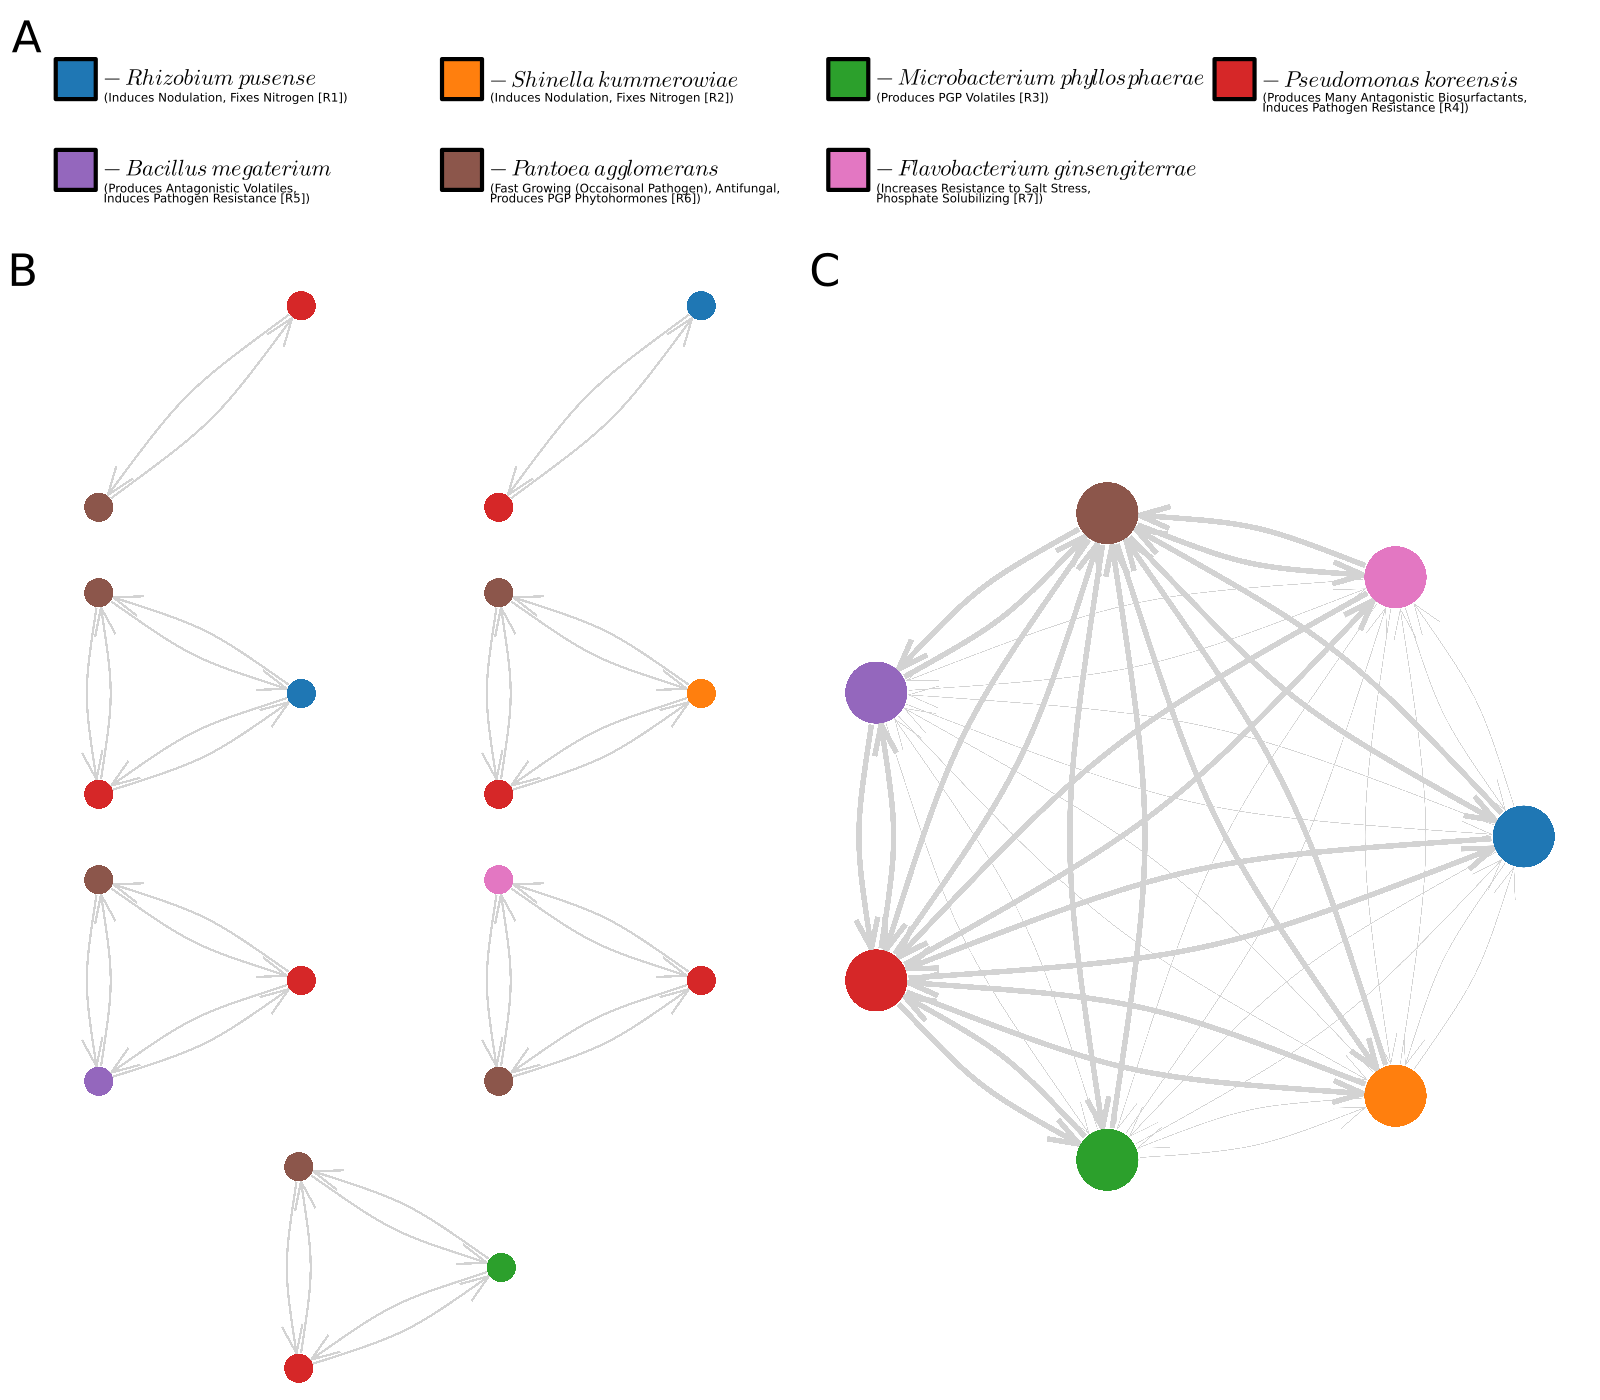
\includegraphics[width=2.0\columnwidth]{figs/Intro_Figure.png}
    \centering
    \caption{\textbf{A.} Legend of species (consistent in all figures) and relevance to rhizosphere microbiome design, \textbf{B.} Subcommunities cultured to parameterize full community model. \textbf{C.} Resulting gLV network approximation (65\% of all parameters). Bold edges represent parameterized interactions and thin edges represent neglected interactions.}\label{fig:intro}
\end{figure*}

In this work, we parameterize the gLV dynamics of a 7-member, synthetic microbial consortia cultured along gradients of environmental backgrounds (Figure \ref{fig:intro}). The community is composed of isolates with 16S regions most closely related to \textit{Rhizobium pusense} (RP), \textit{Shinella kummerowiae} (SK), \textit{Microbacterium phyllosphaerae} (MP), \textit{Pseudomonas koreensis} (PK), \textit{Bacillus megaterium} (BM), \textit{Pantoea agglomerans} (PA), and \textit{Flavobacterium ginsengiterrae} (FG) and were extracted from the rice rhizosphere of plants cultivated in various soil compositions [is there a Colemen-Derr paper?]. Isolates were chosen to include members with genetic similarity to Plant-Growth-Promoting or antagonistic species, members which are frequently abundant in the rhizosphere, as well as members with a range of growth rates. Cultures were grown in a liquid phase and passaged to mimic the continuous recirculating environment of a hydroponic rhizosphere where nutrients are periodically replaced. Subsets of the organisms were grown in pairwise and triwise cultures to parameterize a rigorous model as proved by Venturelli \emph{et al.} 2019. However, we limited subcommunity cultures for parameterization to pairs between the most abundant organisms, and triplicates with those pairs, to minimize the amount of required training data for the model. We show that this amount and type of training data proved sufficient to accurately predict microbiome trajectories in full community cultures along the environmental gradients of temperature and glucose in static and switched contexts. 

We chose to culture the community along two environmental gradients: initial glucose concentration and temperature. It is well known that plants under duress already utilize population-directed environmental control by exuding certain carbohydrates to increase the abundance of PGP species [multi-pseudomonas paper...]. Alternatively, temperature is an easily controlled variable from an engineering standpoint with global effects on chemical kinetics. We hypothesized that a signal like glucose might induce discrete changes in transcription and behavioral strategy, resulting in hybrid system dynamics, while temperature would affect kinetic reaction rates universally and gradually, inciting continuous shifts in the dynamics. Ultimately, the experiments demonstrate how the given microbial community dynamics fluctuate on environmental gradients and stabilize to various diversities, suggesting the significance of an environment based gLV model. 

We use the verified model to explore \textit{in silico} how this understanding could augment microbiome modulation programs in both hybrid and continuous contexts. To theoretically drive the studied synthetic consortia, we use Model Predictive Control (MPC) [Borrelli] as well as Hamilton-Jacobi-Isaacs (HJI) reachability analysis [Tomlin] on the following stochastic gLV formulation,
\begin{equation} \label{ctrl_dist_gLV}
    \dot{x} = x \circ (r + Ax) + Bu + d
\end{equation}
with bounded random disturbance $d \in \mathbb{R}^n$. Both control programs are evaluated
with and without the ability to vary the environment ie. $r$, $A$ and $B$. While limited to simulation, these last analyses underscore the influence of the environment in the design of microbial therapies. Scheduled manipulations of the setting can reduce the necessary quantity of input as well as increase the radius of treatable states making control more efficient and powerful.

\section*{Experimental Design}

\indent \indent Pairwise co-culture parameterization of gLV models results in high fidelity predictions of dominating species [Venturelli]. In contrast, attempting to fit $n \geq 3$ systems with only full community data can suggest equally predictive parameter sets that yet vary in response to perturbations. Note, the gLV model is a single layered neural network, famous for their tremendous flexibility as approximators. While more reliable however, pairwise fitting is expensive. The number of pairs grows with $\mathcal{O}(n^2)$ and each pair requires multiple time-points, which need to be processed to identify diversity and total abundance. With prior knowledge of full-community diversity, it is possible to compromise experimental labor with model fidelity. The affect and rate of change of a population is magnified by its size. Thus, rare species generally have lesser influence and interactions between them are less relevant. We used this principle to guide the selection of training data.

The gLV model is fit with data from isogenic cultures, from two of the three pairs between the three most abundant members, and from triples between the two most abundant members and a rare member (Figure \ref{fig:intro}). This set allows fitting of $65\%$ of all parameters, including growth rates $r$ for each species, with 14 rather than 28 cultures (total pairs). The model is validated by attempting to predict the growth of full community cultures in both static and switched environments where glucose concentration or temperature is changed on 48-hour schedules. 

All organisms were grown to an OD of 0.2 before being combined in equal proportion to make the pairs, triplets, and full community cultures. All cultures were grown in triplicate in 2mL of 10\% TSB, inoculated with a combined OD of 0.001, and passaged after 48 hours with 1:20 dilution, twice (144 hours total). On 24 hour intervals, 200 uL was removed for OD and 400 uL was removed to spin down (prior to passaging). For cost and simplicity, the Direct PCR method [Fangchao] (Supplemental) was used to extract genomic DNA from the centrifuged biomass and subsequently amplified with double-barcoded 16s primers [Morgan, Adam D] to allow all samples to be pooled prior to sequencing. 

The sequencing results were processed with Perl scripts to extract counts of 16s populations as described in [Price] and then aligned, quantified and organized in Python. The sample's relative abundances were computed from the counts and then multiplied with the corresponding OD sample to generate absolute abundance, time course data used for training the gLV model. 

\section*{Parameterization}

The gLV model for each of the 8 conditions is trained via a two part global-local optimization strategy. We had best success generalizing from the training to the full community data by training with an adaptive differential evolutionary algorithm (ADE) in both legs [BlackBoxOptim], although several well-known gradient based were tried. The success of this method might be due to the relatively low ratio of timepoints to parameters being fit, rather than the nature of the gLV though. In addition, to counter the gLV's hyper flexibility and elucidate the underlying biological phenomenon, a penalty on the deviation between condition-adjacent fits was included to encourage a parsimonious difference in parameters. With respect to the dynamics, the simulations are initialized from the first data point to skirt the stochasticity of communtiy establishment [Justice] and also include the discrete event of $1:20$ passaging on 48 hour intervals.

The global and local optimization programs share the same loss function but are initialized from different positions in the state space. The global run is initialized with random populations spanning the parameter ranges listed below, but with growth rates and self interactions centered on estimates made from the isogenic final points. The local run is initialized with the optimal solution of the global run and uses parameter ranges which are within $50\%$ of the previously optimal value. The loss function for both legs iterates over all subcommunity cultures (singles, pairs and triplets) to sum a total cost. This allows parameters which are utilized in multiple subcommunities to be fit to multiple experiments simultaneously. All parameterization scripts were written in Julia [JuliaLang].

The loss is defined as the replicate-averaged, sum L2 norm between observed states $x_t$ and gLV predicted $\hat{x}(t)$ for time points $t \in t_p$ with L1 regularization on the parameter set and between condition-adjacent parameter sets. Thus, the loss takes the form,
\begin{equation} \label{loss_global}
    L(p) = \mathlarger{\sum}_{s \in S} n_r^{-1}
    \mathlarger{\sum}_{x_0 \in R_0}
    \mathlarger{\sum}_{t \in t_p}
    \left\lVert x_t - \hat{x}(t) \right\rVert_2 
    + \gamma_1 \left\lVert p \right\rVert_1
    + w
\end{equation}
where $p$ is the flattened vector of gLV parameters $r$ and $A$, $S$ is the set of all subcommunities, $R_0$ is the set of initial states of each replicate, $n_r$ is the number of replicates for each subcommunity, $\gamma_1$ is the regularization coefficient, and $w$ is the deviation penalty. We chose to fit the lowest environment value case with $w = 0$ and then for each increase in glucose or temperature $w$ becomes the weighted norm between the parameters being fit $p$ and the previous fit's parameters $p_c$,
\begin{equation} \label{deviation_penalty}
    w = \begin{cases}
        0, & \text{0.31mM glucose or $25 ^{\circ}$ C} \\
        \gamma_2 \left\lVert p - p_c \right\rVert_1, & \text{else}
      \end{cases}
\end{equation}
\noindent Hence, the loss encourages the fits to differ in a minimal number of parameters from one another. This method was chosen over direct gradient descent from one set to another to avoid the implicit assumption that the basins of the minima overlap.

\begin{figure*}[!ht]
    \centering
    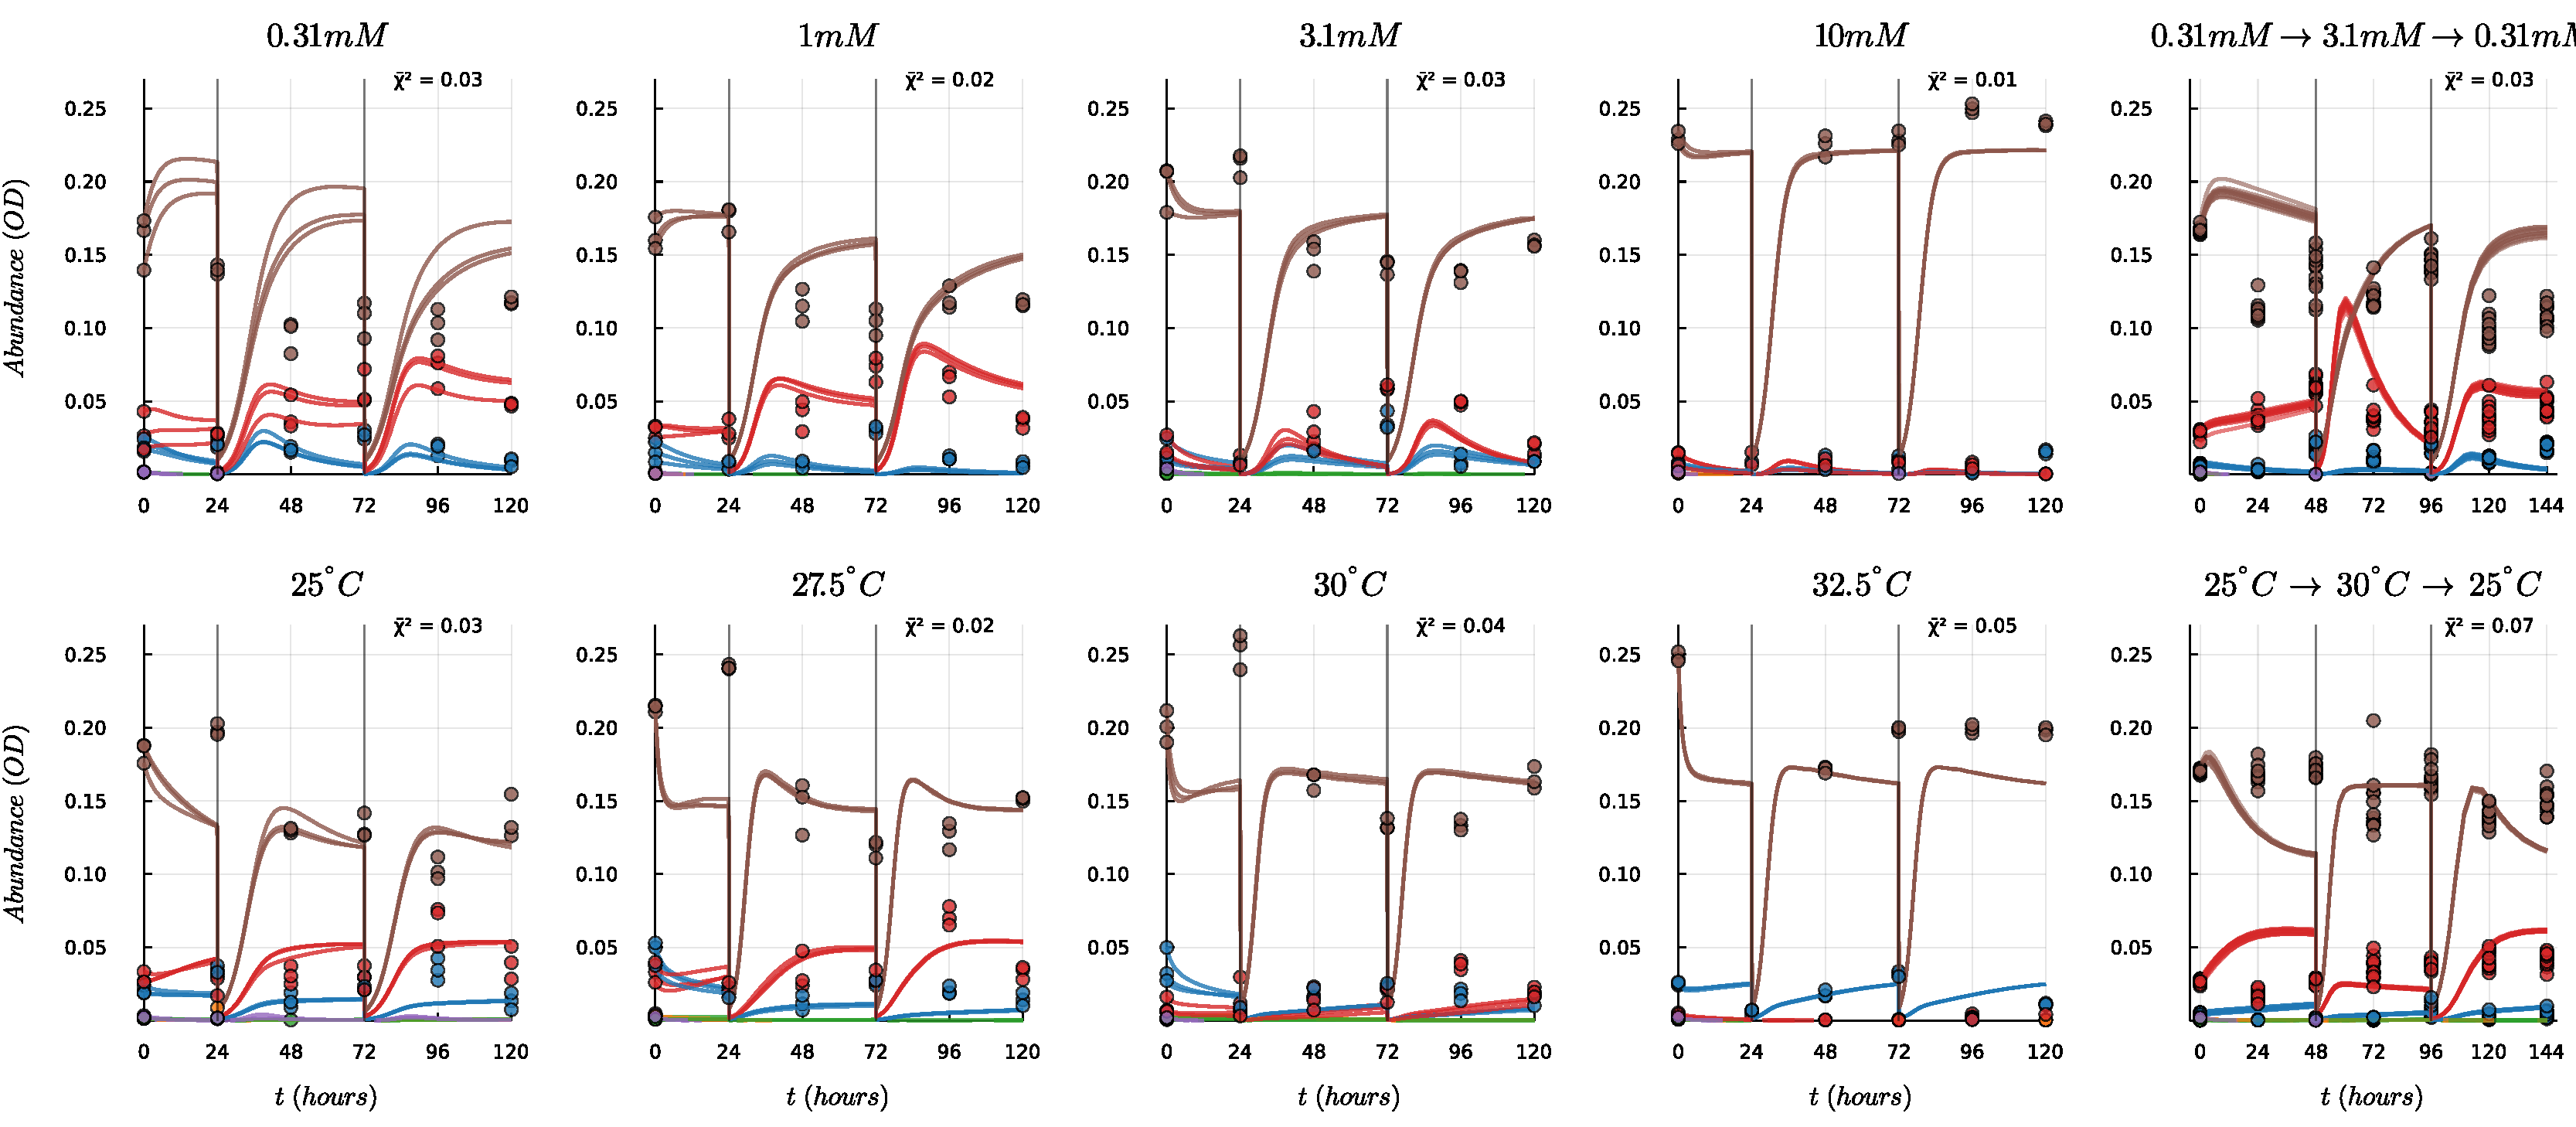
\includegraphics[width=2.0\columnwidth]{figs/model_validation.pdf}
    \centering
    \caption{\textbf{Model Validation with Best Fit} Data (circles) vs. simulations (lines) of full-community systems in static or switched environments. Mean goodness-of-fit $\bar{\chi}^2$ for all species and replicates listed in the upper right corner.}\label{fig:mv}
\end{figure*}

% The direct loss for the local leg is similar but replaces the L2 with the normalized sum squares between predicted and observed states, identical to the $\chi^2$ goodness-of-fit. This amplifies small-dimension error to correct low-abundance species predictions. Thus, the total loss for the local leg takes the form,
% \begin{equation} \label{loss_local}
%     L_{l}(p) = \mathlarger{\sum}_{s \in S} \frac{2^{n_s}}{n_r}
%     \mathlarger{\sum}_{x_0 \in R_0}
%     \mathlarger{\sum}_{t \in t_p}
%     \mathlarger{\sum}_{i \in N}
%     \frac{(x_{i,t} - \hat{x_i}(t))^2}{|x_{i,t}|}
%     + \gamma \left\lVert p \right\rVert_1
%     + w
% \end{equation}

% In summary, first, either $0.31mM$ glucose or $25 ^{\circ}$C are fit with the ADE which generates a population of random vectors within the chosen parameter bounds of $r_i \in [0.05, 1.0]$, $\alpha_{ii} \in [-3.0, -0.25]$, and $\alpha_{ij} \in [-3.0, 3.0]$. These parameters are iteratively scored with (\ref{loss_global}) and bred for $1e6$ function calls. This process is repeated for the other environmental condition gLV systems for $1e5$ calls. With several independent runs, a localized search bounds is computed with $20\%$ padding. Finally, we initialize the ADE again within the confined range with the normalized loss function and optimize (\ref{loss_local}) for the same quantity of iterations for each condition. All growthThe final fit of all training data can be viewed in the supplemental (Figure \ref{fig:mf}).

\begin{Figure}
    \centering
    % 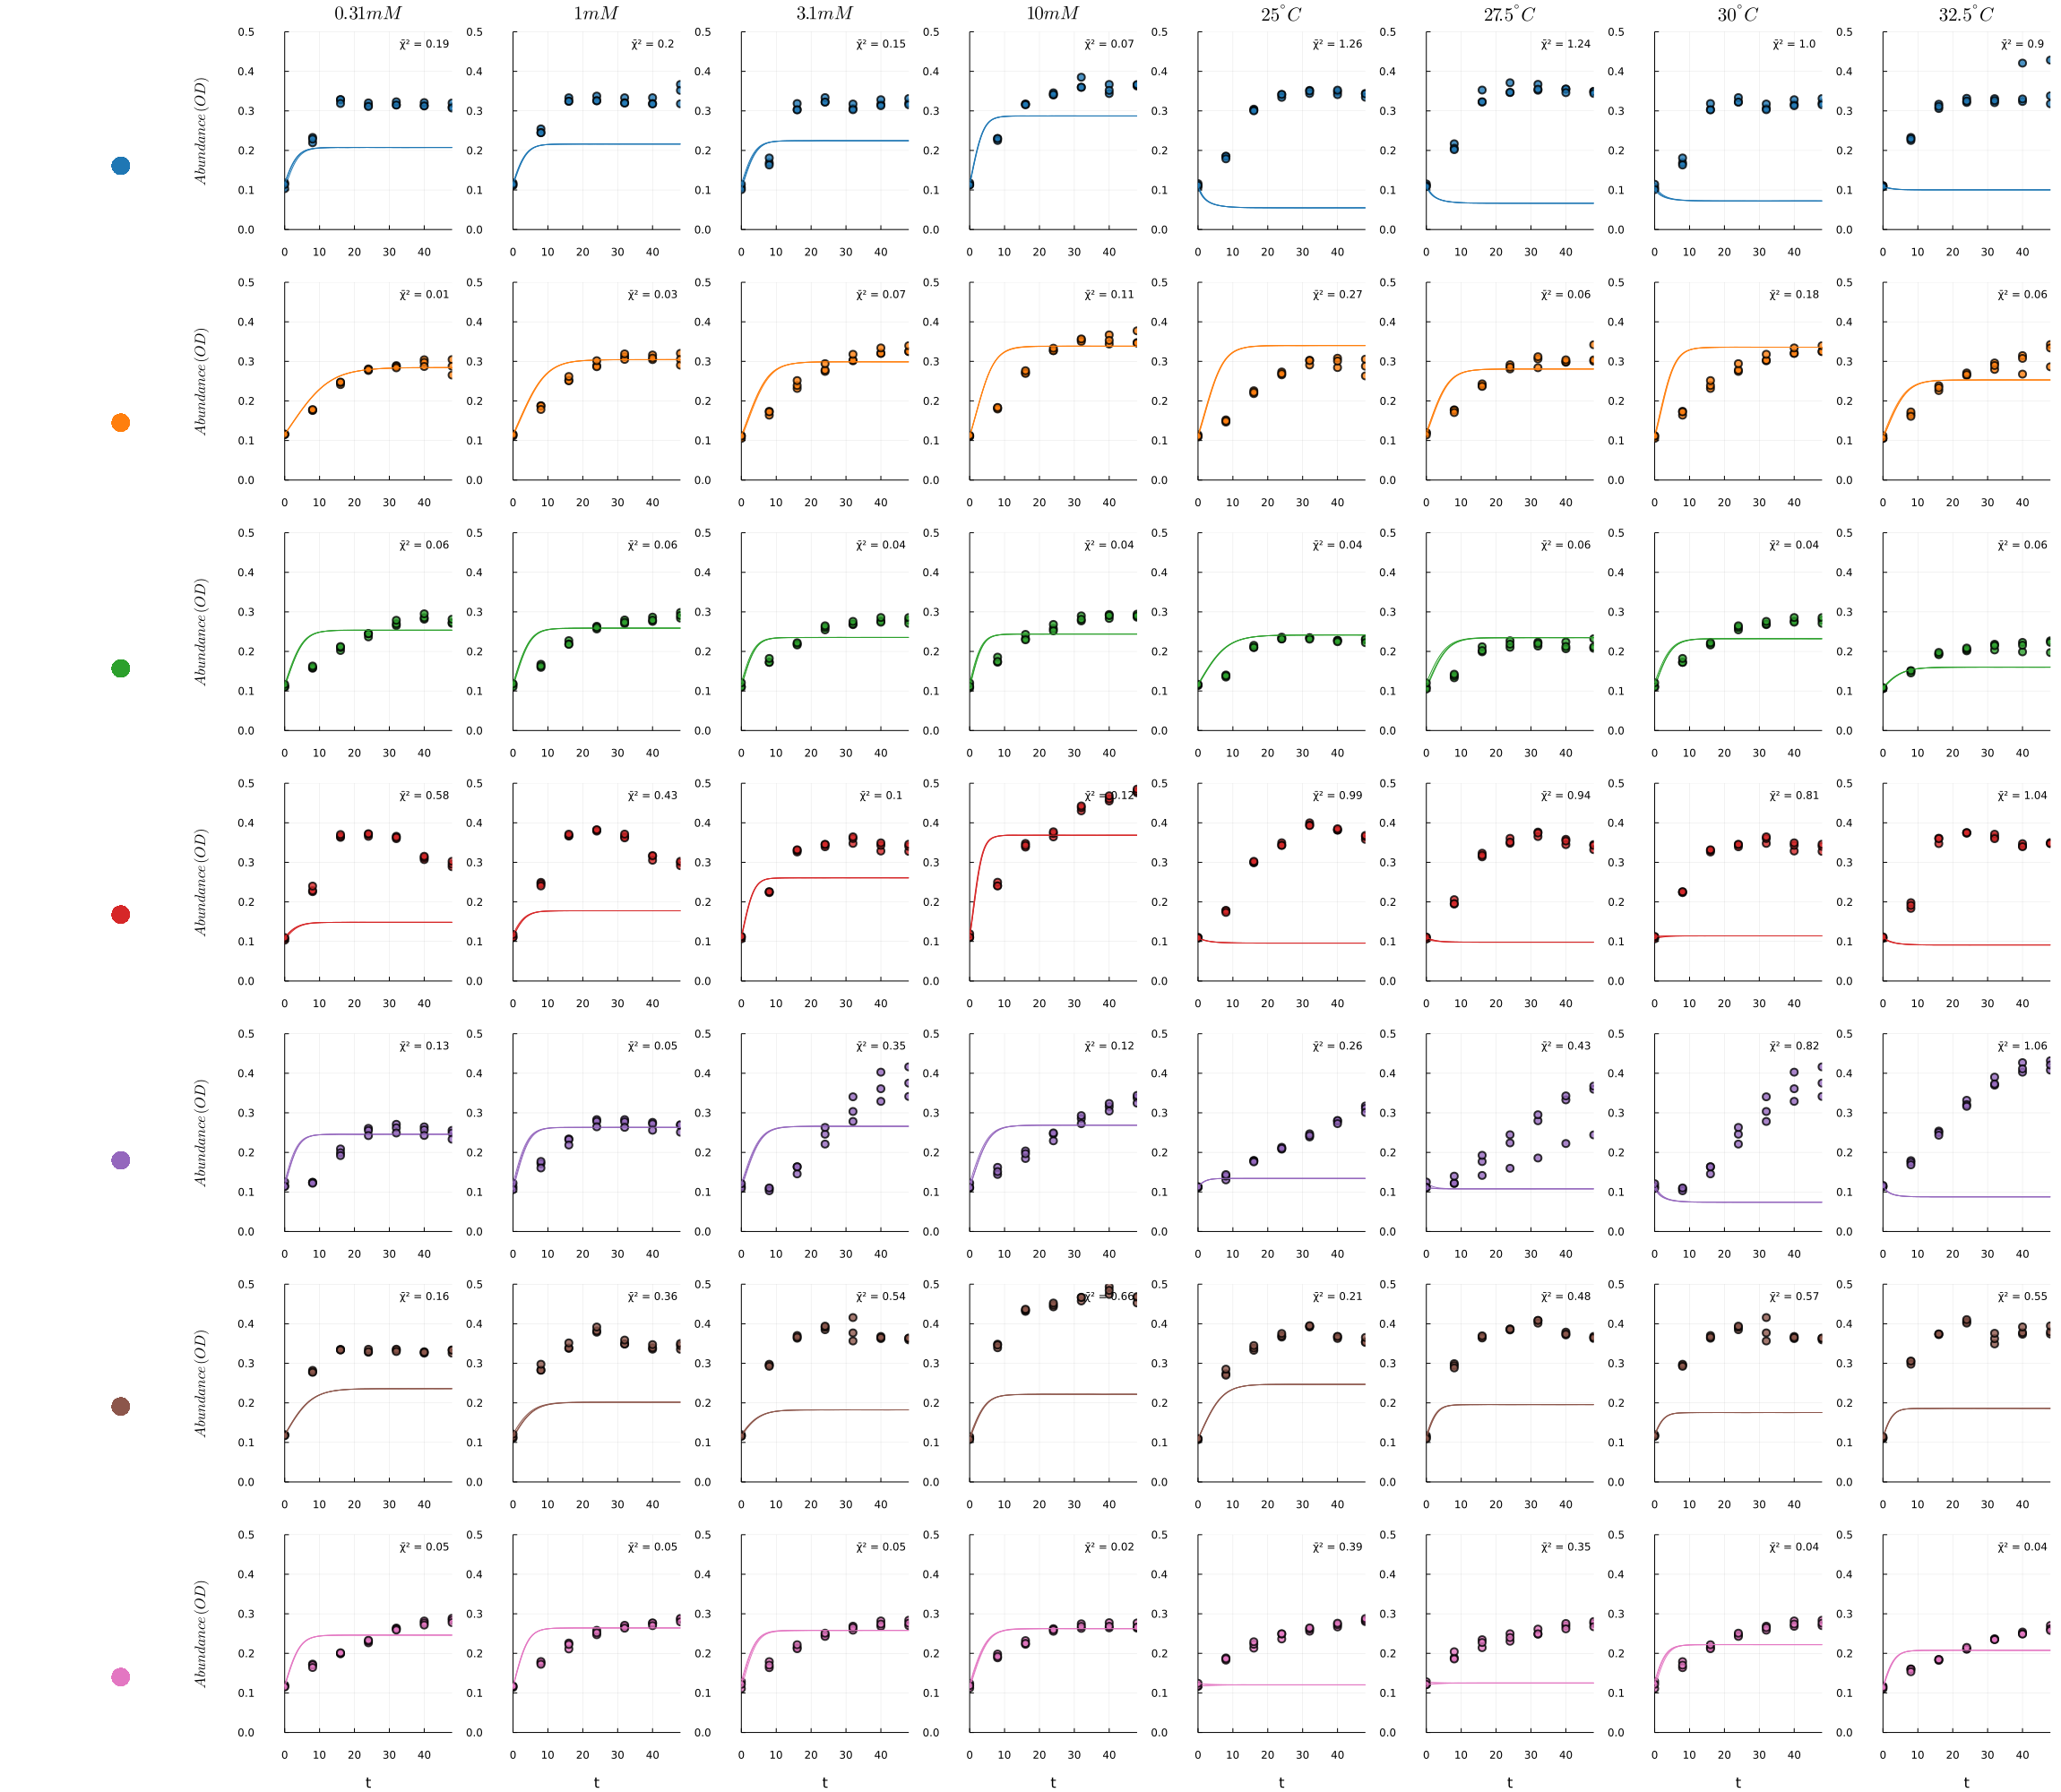
\includegraphics[width=1.0\columnwidth]{figs/model_fit_iso.pdf}
    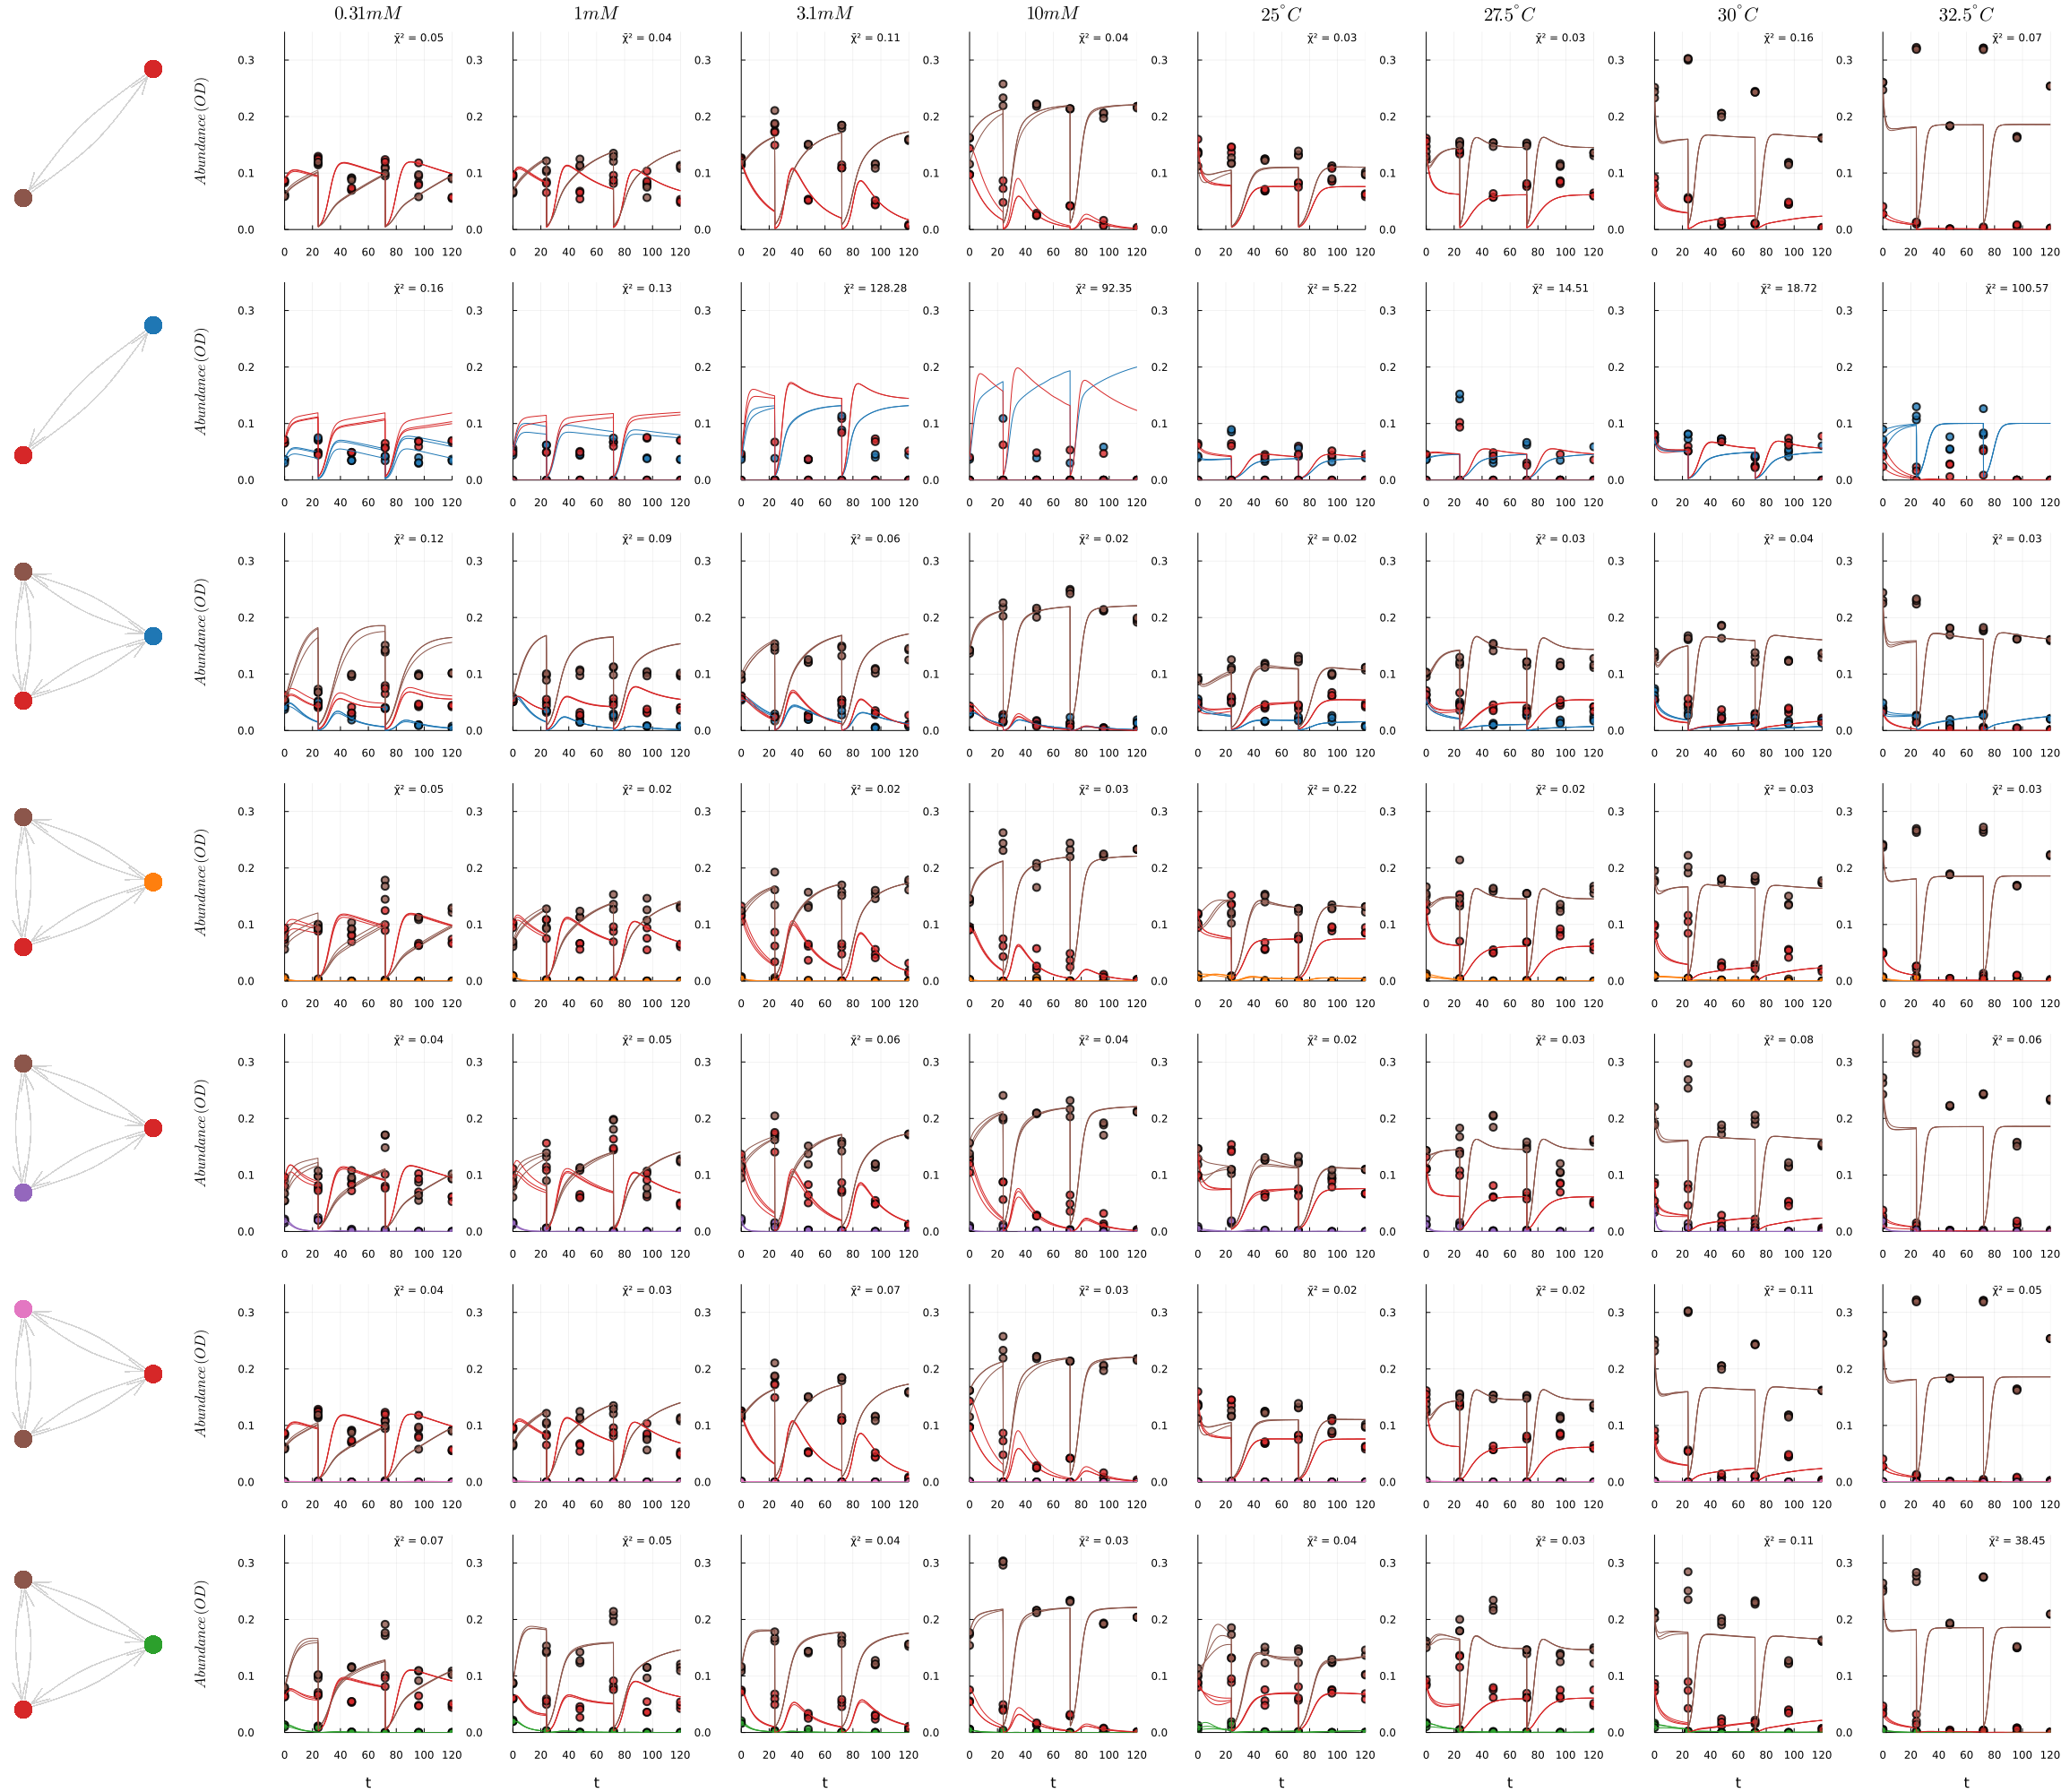
\includegraphics[width=1.0\columnwidth]{figs/model_fit.pdf}
    \centering
    \captionof{figure}{\textbf{Model Fit on Training Data} The best fit compared with the training data of all isogenic cultures. Real timecourse data are depicted as circles and model prediction is depicted as continuous lines.}\label{fig:mftd}
\end{Figure}

The training data (points) and best model fit (smooth lines) are displayed in the grid above, with rows and columns ordered by subcommunity and environmental condition (\ref{fig:mftd}). In most subcommunity cultures, PK and PA dominate the absolute abundance, occupying $> 90\%$ of the diversity, despite significant growth in isogenic contexts by all species.

\subsection*{Model Analysis}

The trained model predicts the full community trajectories with $\bar{\chi}^2) = 0.026$ \& $0.042$ for glucose and temperature gradients respectively. Remarkably this was done with data for only half the cultures compared to the full pairwise parameterization. The microbiome at hand converges to states where isolates closely related to PA, PK and RA occupy $\geq 99\%$ of the total diversity while members SK, MP, BM transiently appear at $0.1$ to $1\%$ and FG appears at $< 0.1\%$. At higher glucose concentration and temperature, the diversity drops and PA further out-competes PK and RA leaving a nearly isogenic microbiome. The strength of the parameterized model suggests that differences in population dynamics across these environmental gradients are explained by species changes in ecological interactions between one another and with themselves.

\begin{figure*}[!ht]
    \centering
    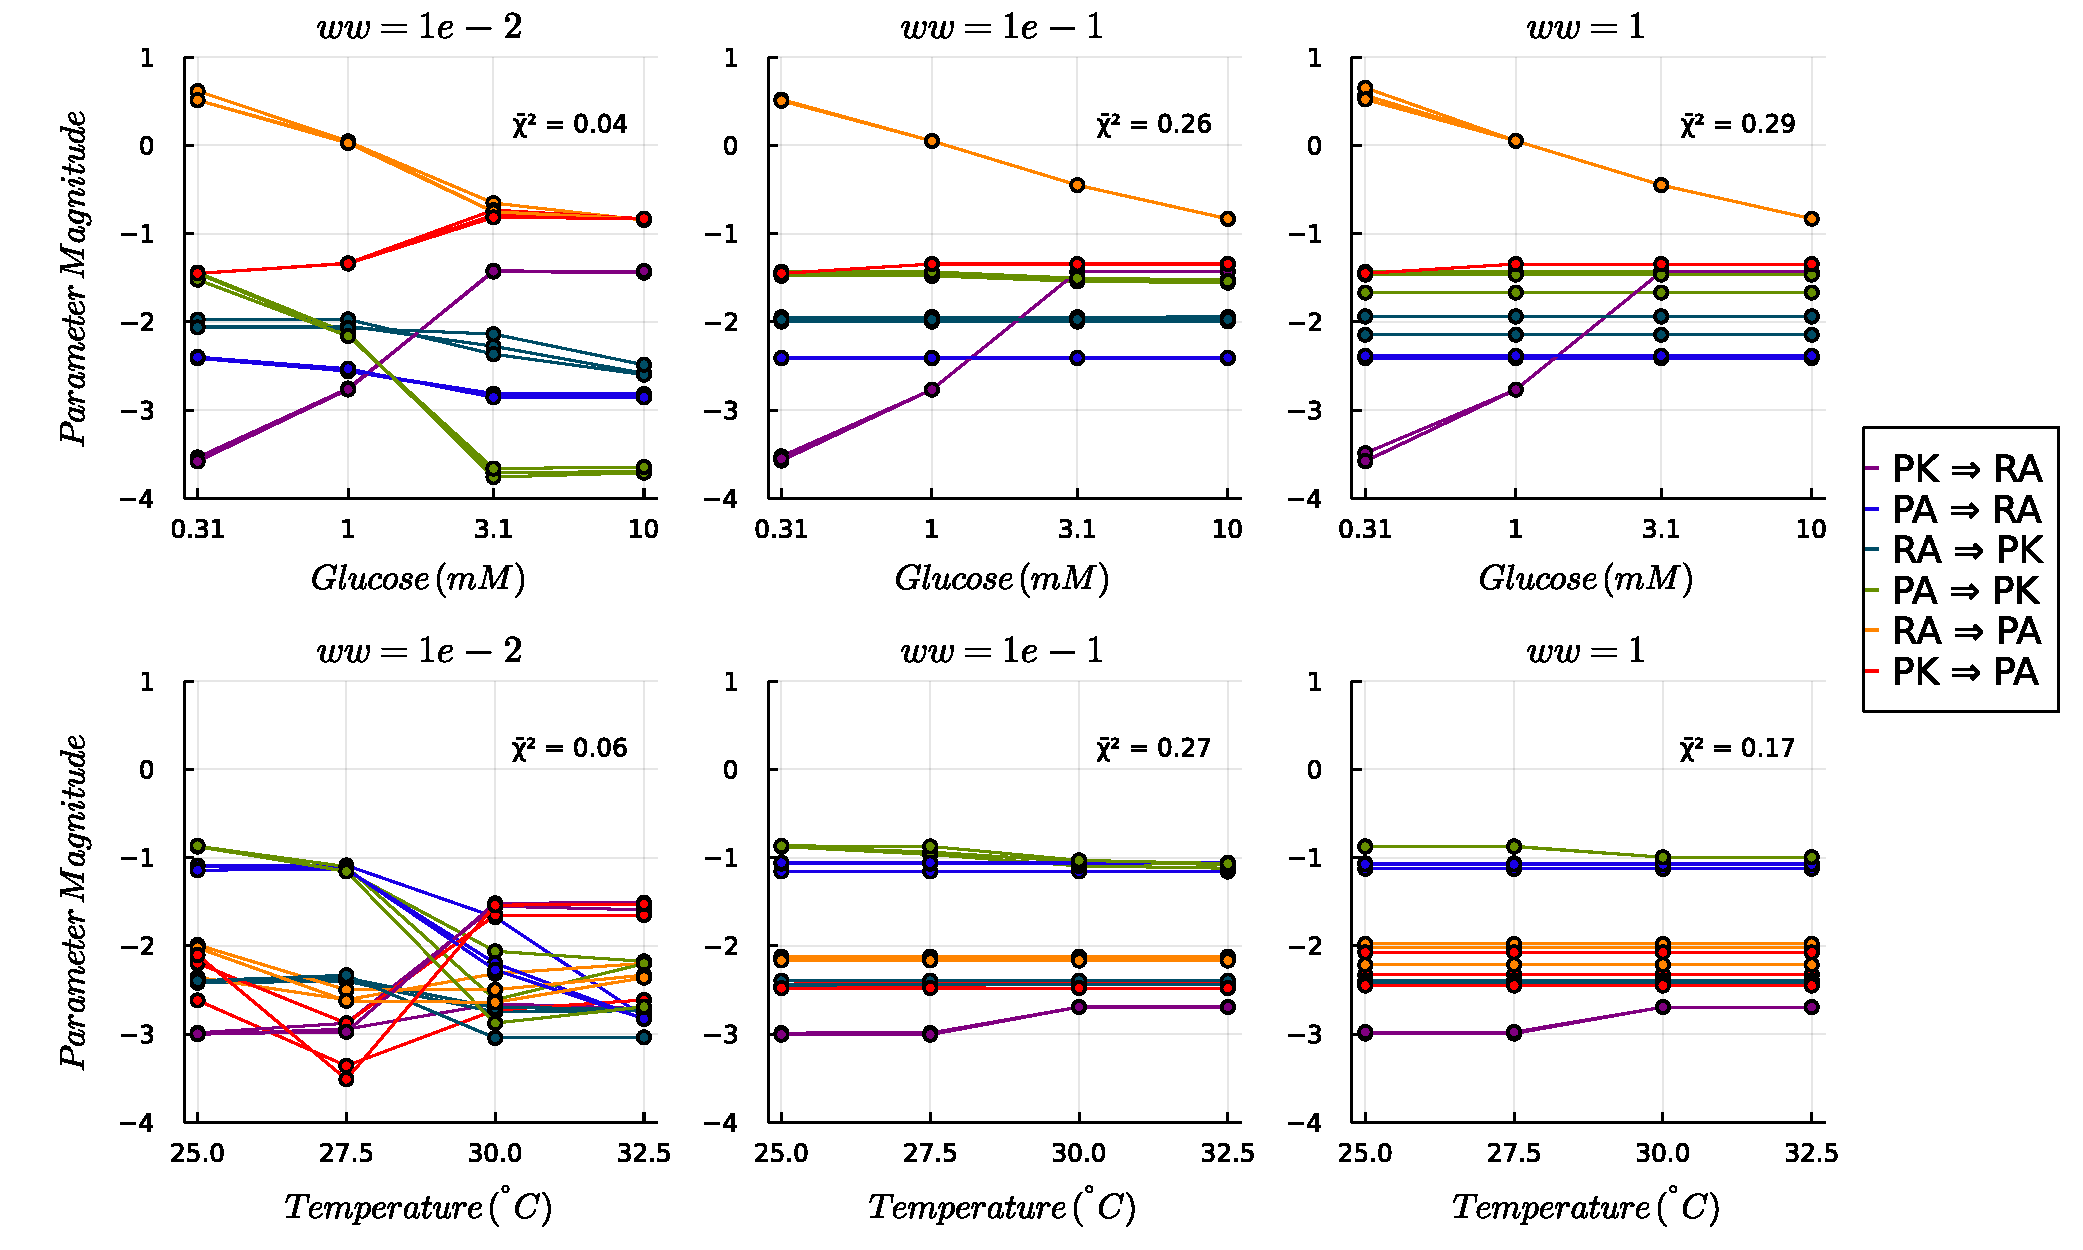
\includegraphics[width=2.0\columnwidth]{figs/intrxns_over_wwfits.pdf}
    \centering
    \caption{\textbf{Principle Interaction Variance over Model Ensemble} Three parameter outputs of principle inter-species relationships are displayed for three different wander regularization penalties for both glucose and temperature settings. Opacity corresponds to $1 - \bar{\chi}^2$ of the given fit.}\label{fig:iv}
\end{figure*}

Of the pairwise data, variation over environmental gradients is most noticeable between members PK and PA (Figure \ref{fig:mftd}). At lower glucose and temperature, the two species balance one another and, across replicates, the relative abundance tightly oscillates around a 1:1 equilibrium. However, as glucose concentration or temperature increases, the oscillations diverge and PK yields to PA by 144 hours, despite that both have improved growth in the corresponding isogenic settings (Figure \ref{fig:mftd}). While not true for all species, the outcome of these two principal members matches the ranking of their isogenic growth rates and final abundances in all environment settings. The best-fit model captures this with $r_{PA} > r_{PK}$ and suggests that strong negative pressures $\alpha_{PA-PK}$ and $\alpha_{PK-PA}$ allow one another foothold. Despite that this work abstains from a molecular resolution of interactions, it reiterates the previously postulated principle that the best competitive advantage is rapid and massive growth. This would explain why the continuous tuning of growth-relevant environmental variables results in a smooth slide of the fixed point diversity in the full community. This trend might fail if a given species massively altered its genetic program but this is not observed in the given time frame or environments.

Over an ensemble of fits, numerical optimization suggests that a few interactions are responsible for the fluctuation in dynamics. Given the aforementioned nonlinearity of the objective function, stochastic optimization can yield solutions in a diversity of local minima with similar loss. Thus, an ensemble of models - garnered from different runs of the evolution algorithm - is compared to identify key changes in the parameter set over the environmental gradients (\ref{fig:iv}). The evolutionary algorithm employed tends to find similar local minima under fixed regularization parameters but is sensitive to the wander penalty. The wander penalty acts as an L1 regularization on the change in parameter set and, thus, the higher the weight, the more sparse the vector defined by the difference in any two sets. Under the largest penalties, parsimony in the variation highlights the importance of the PK->RA, RA->PA, and PA->PK interactions to explain the overall change in dynamics. Overall, the model suggested that almost all interactions were negative in this synthetic soil community which agrees with previously studied soil communities [Morgan knew of a paper?].

Interestingly, interactions became more antagonistic as glucose concentration rose. In this community, rather than observing a battle of scarcity, the best-fit model suggests organisms became aggressive as one member, PA, began to take larger footholds in the community. This agrees with the isogenic data which demonstrate that PA grows exceptionally at the higher glucose concentration but is withheld in the corresponding setting when RA and PK are present. Although, we cannot make causal inferences from the modelling, this continues to underscore that changes in inter-species interactions correspond with changes in a populations individual relationship with its environment. It also suggests that maybe if the change in an environment doesn't injure or encourage any individual population's growth, relationships will remain static, but this remains future work.

\indent \indent The non-trivial equilibria of the autonomous gLV system satisfy either of the following equations,

\begin{minipage}{0.42\linewidth}
    \begin{equation}
        Ax = -r \label{full_fp}
    \end{equation}
\end{minipage}%
\begin{minipage}{0.42\linewidth}
    \begin{equation}
        A_{s}x = -r_{s} \label{sub_fp}
    \end{equation}
\end{minipage}

\hspace*{1cm}

\noindent for any subcommunity $S:[1, n] \mkern7mu \backslash \mkern5mu \{i\}$ where $x_i = 0$. While full-community fixed points often include negative values for specific states, in the bounded system the trajectory is intercepted at the $x_i = 0$ subspaces resulting in a subcommunity without member(s) $i$. Furthermore, in systems with scheduled resets (eg. due to passaging), hybrid limit cycles may appear where reset trajectories jump into regions of stability where they previously converged. As demonstrated by Gore et al., in the continuous case as well, dilution can similarly create alternative stable states [Gore]. 
 
It's clear from the experiments that the microbiome at hand rapidly converges to the three dimensional subspace of \textit{PA}, \textit{PK} and \textit{RA}, however, the 120-hour final point of this subsystem shifts from a rich diversity at low glucose and temperature to a \textit{PA}-dominated system at high glucose and temperature [Figure 4a,b]. The best-fit model suggests that the systems are indeed converging to fixed points with varying diversity as well as varying stability, which become trapped in limit cycles near these fixed points. Interestingly, the best-fit model predicts that several of these limit cycles capture unstable subcommunities in loops and otherwise converge to an isogenic systems if simulated without dilution. The rate of convergence in these scenarios is due to the dominating fixed point when left without passaging. The minimum eigenvalue of the Jacobian at each of these equilibria, given by,
\begin{equation} \label{jacob}
    D_{x}f(x,r,A) = Diag(r + Ax) + Diag(x)A
\end{equation}
is used as a measure of the rate of convergence and these are computed for each environmental condition (Figure \ref{fig:roc}). These plots illustrate that over the ensemble of fits, the minimum eigenvalue magnitude rises indicating that the rate of convergence is faster for both higher glucose and temperature. Hence, lower glucose and temperature systems will take many passages (or potentially seasons) to converge to a limit cycle. The variation in rate of convergence at all is exciting from the perspective of control as it offers different playing fields for manipulating the system. Generally, faster systems are more difficult to manipulate, however, there might also be situations where we would like to accelerate the progression. This finding is interesting and suggests that there may be useful reasons to complicate modulation programs of a microbiome. We will explore this in simulation in the second half of the work.

\begin{figure}[!ht]
    \centering
    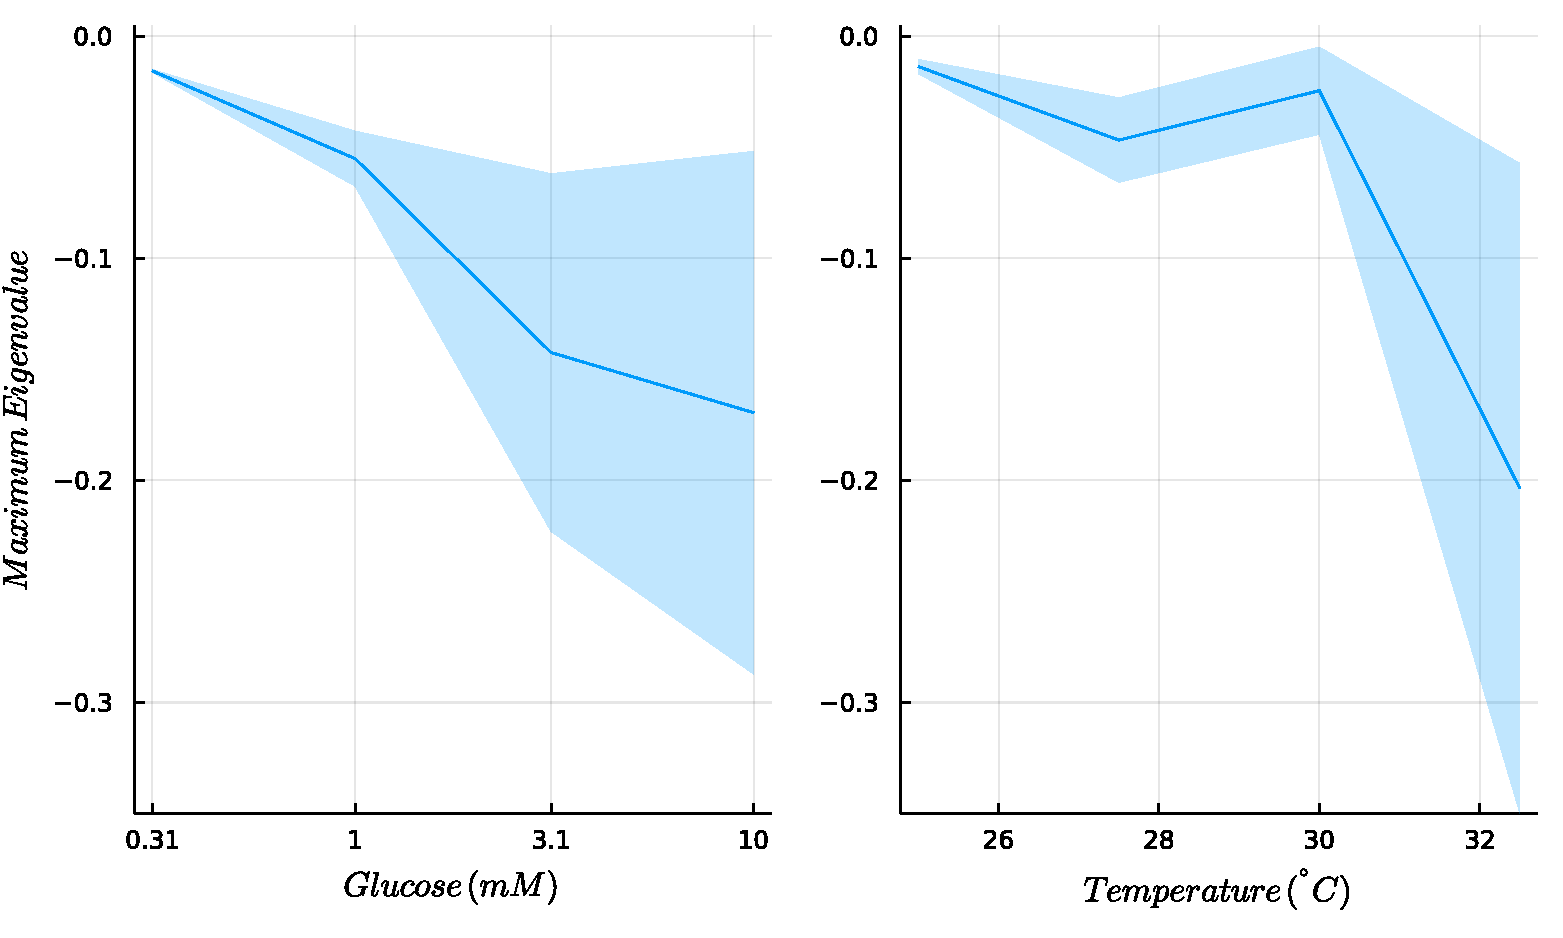
\includegraphics[width=1.0\columnwidth]{figs/ROC_change.pdf}
    \centering
    \caption{\textbf{Rate of Convergence over Environmental Gradients} Average minimum eigenvalue magnitude over the model ensemble is plotted for each glucose and temperature condition.}\label{fig:roc}
\end{figure}

\section*{Theoretical Modulation of Environment-varying gLV Systems}

\indent \indent With the parameterized microbiome model, we consider the problem of controlling a gLV system \textit{in silico} with and without environmental fluctuation. We consider the dynamics of only the $3$ most abundant members with consistent representation in the diversity. The potential to control both temperature and glucose models is analyzed in the context of driving the microbiome to the following subcommunity equilibria: the \textit{PA-PK-RA} fixed point, \textit{PA-PK} fixed point, \textit{PA-RA} fixed point, and the \textit{PK-RA} fixed point. This problem is inspired by the seasonal or situational need to select for different diversities attributed to certain agricultural benefits. While the data show that the full 3-membered equilibrium is stable, we include this target to gauge how environmental control can slow or quicken convergence.

We simulate the forward perspective of driving the microbiome with a linearized Model-Predictive controller from one equilibrium to another, and we compute and analyze the Backwards Reachable Tube (BRT) [Tomlin] for a given equilibria in time $\tau$ with a Hamilton-Jacobi-Isaacs controller. The former is used for analyzing a continuous temperature model and the latter for a hybrid glucose model. The linearized MPC is a fast algorithm which has proved successful in the true nonlinear gLV dynamics [Angulo et al.], but stochasticity can impede success and MPC methods for nonlinear, hybrid systems are limited. Backwards-reachability is valuable for determining the boundary set of states which can be driven to an equilibrium under true stochastic, nonlinear dynamics, however, as a dynamic programming method it suffers in high-dimensional systems. Therefore, in the BRT analysis, we are restricted to considering limited schedules of hybrid-state switching and only the case of driving to the 3-membered equilibrium.

Input to disturbance bounds are chosen to be $16\%:8\%$ of the real maximum abundance ($0.3$) to simulate either a recalcitrant system or a cautious modulation program,
\begin{equation}\label{u_d_bounds}
    \lvert u_i \rvert \leq 0.05, \lvert d_j \rvert \leq 0.025
\end{equation}
Furthermore, we simulate all control programs with the full actuated input configuration as well as all pair and single input configurations.

Despite that changes in population dynamics appear similar for both environmental gradients, we assume that because the underlying signals themselves differ two models with two distinct formulations are necessary. With respect to the problem of fitting nonlinear gLV systems, one might choose a hybrid formulation because it restricts control to parameter domains where the models were trained unlike the continuous formulation which requires interpolation between fits. Ultimately, the two methods are demonstrated to offer different control approaches to various types of environmental signals and were selected here based on the nature of glucose and temperature.

\subsection*{Continuous Control of Temperature-Varying Systems}

\begin{figure*}[!htb]
    \centering
    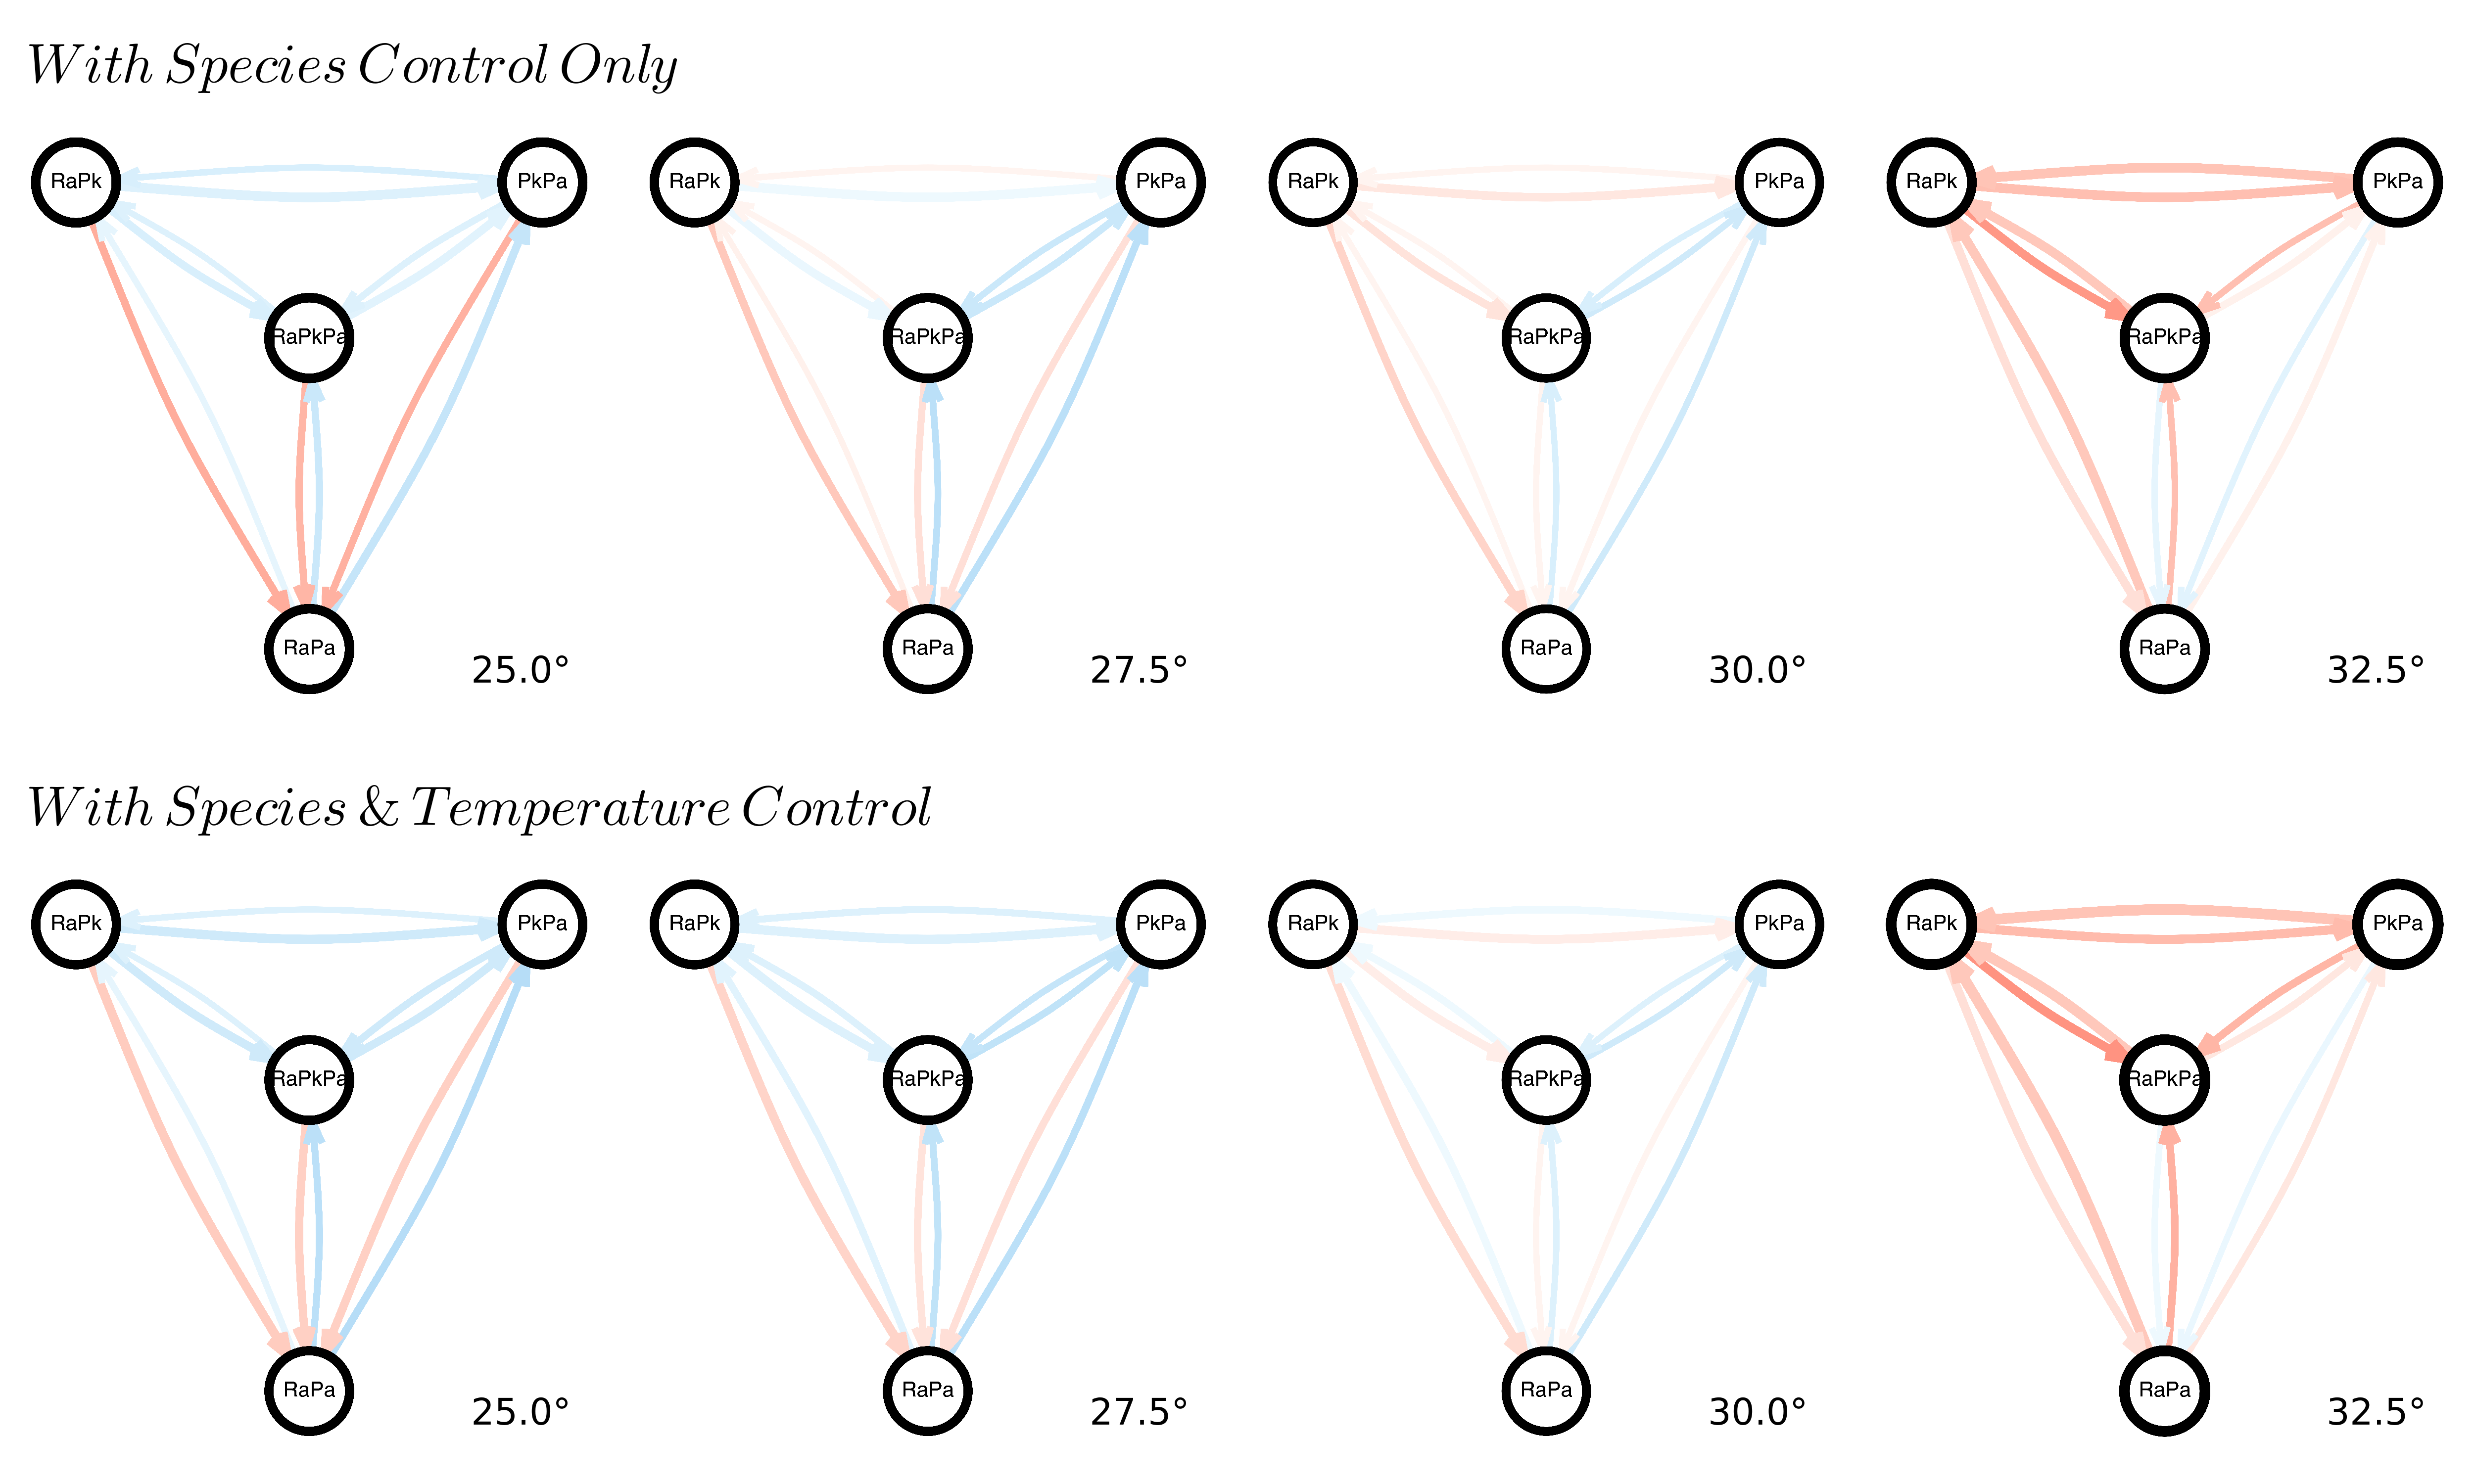
\includegraphics[width=2.0\columnwidth]{figs/MPC_Paths_Figure_Ricatti_hq.png}
    \centering
    \caption{\textbf{Path Success of MPC} Directed graphs depicting the initial-to-target paths the MPC was tested on and the final distance to target (edge color) and total species input (edge width) of the linearized MPC with and without the control of temperature, averaged over all possible control species sets. }\label{fig:mpc_paths}
\end{figure*}

\indent \indent From an engineer's perspective, temperature is an easily controlled variable. It is relatively unperturbed by the microbiome state itself and can be manipulated externally with accuracy. Importantly, it remained constant in the parameterization experiments. For these reasons, we make the assumption that for the experimented window of temperature change, polynomial regression can capture the chemical changes that cause parameter changes. This allows us to consider the problem of driving microbiomes in temperature-varying models with frequent manipulation of temperature (continuously or with $\Delta t=0.1$ intervals). We assume that the dynamics of stabilizing heat loss to a specific temperature are rapid and negligible compared to the gLV timescale (hours), thus the temperature-extended gLV system takes the form,
\begin{align} \label{T_ctrl_dist_gLV}
    \begin{array}{l}
        \dot{x} = x \circ (r(T) + A(T)x) + Bu + d \\
        \dot{T} = u_T \\
        u_T \in [-10, 10]
    \end{array}
\end{align}
where $r(T)$ and $A(T)$ are the 4-degree polynomial regressions of the temperature-parameter mapping and $u_T$ is temperature input. $u_T$ is bounded such that we might raise the temperature $2.5^\circ C$ in $0.25$ hours.

The general quadratic MPC program is used [Borrelli] with the linearized dynamics of the gLV-Temperature extended system with augmented state and input vectors $\hat{x}$ and $\hat{u}$. The MPC objective function penalizes the state and input paths, $\hat{X}$ and $\hat{U}$, by the distance to the target point $\hat{x}_d$ running state-cost matrix $Q$ and running input-cost matrix $R$. Thus, for the full state vector $\hat{x} := [x; \; T]$ and input vector $\hat{u} := [u; \; u_T]$ with path matrices $\hat{X} := [\hat{x}_1, \dots \hat{x}_h]$ and $\hat{U} := [\hat{u}_1, \dots \hat{u}_h]$, the nonlinear program seeks to minimize,
\begin{align} \label{MPC_cost}
    \begin{array}{c}
        \min\limits_{\hat{X},\hat{U}} \mathlarger{\sum}_{k=1}^{h} \left\lVert \hat{x}_k - \hat{x}_d \right\rVert^T Q \left\lVert \hat{x}_k - \hat{x}_d \right\rVert + \left\lVert \hat{u}_k \right\rVert^T R \left\lVert \hat{u}_k \right\rVert 
    \end{array}
\end{align}
subject to the aforementioned state constraints and Forward Euler dynamics constraints,
\begin{align} \label{MPC_dyn_con}
    \begin{array}{c}
        x_{i,k+1} = max(0, \;  x_{i,k} + \Delta t*\dot{x}_{i,k}) \\
        T_{k+1} = T_k + \Delta t*\dot{T}_k
    \end{array}
\end{align}

Performance of the MPC is scored on two metrics: final species distance, the L2 distance between the final and target states after 6 hours of MPC action, and normalized total species input, the absolute sum of probiotic/antibiotic input during the program normalized by the number of species in the input configuration. While several solvers exist for Linear Finite Time Optimal Control (LFTOC) problems of this type, in simulation, mapping the discrete algebraic Ricatti solution of the unconstrained problem to the above state bounds resulted in a controller that significantly outperformed the LFTOC solutions with 1000x faster runtime [I can put this plot in supplemental].

\begin{figure*}[!htb]
    \centering
    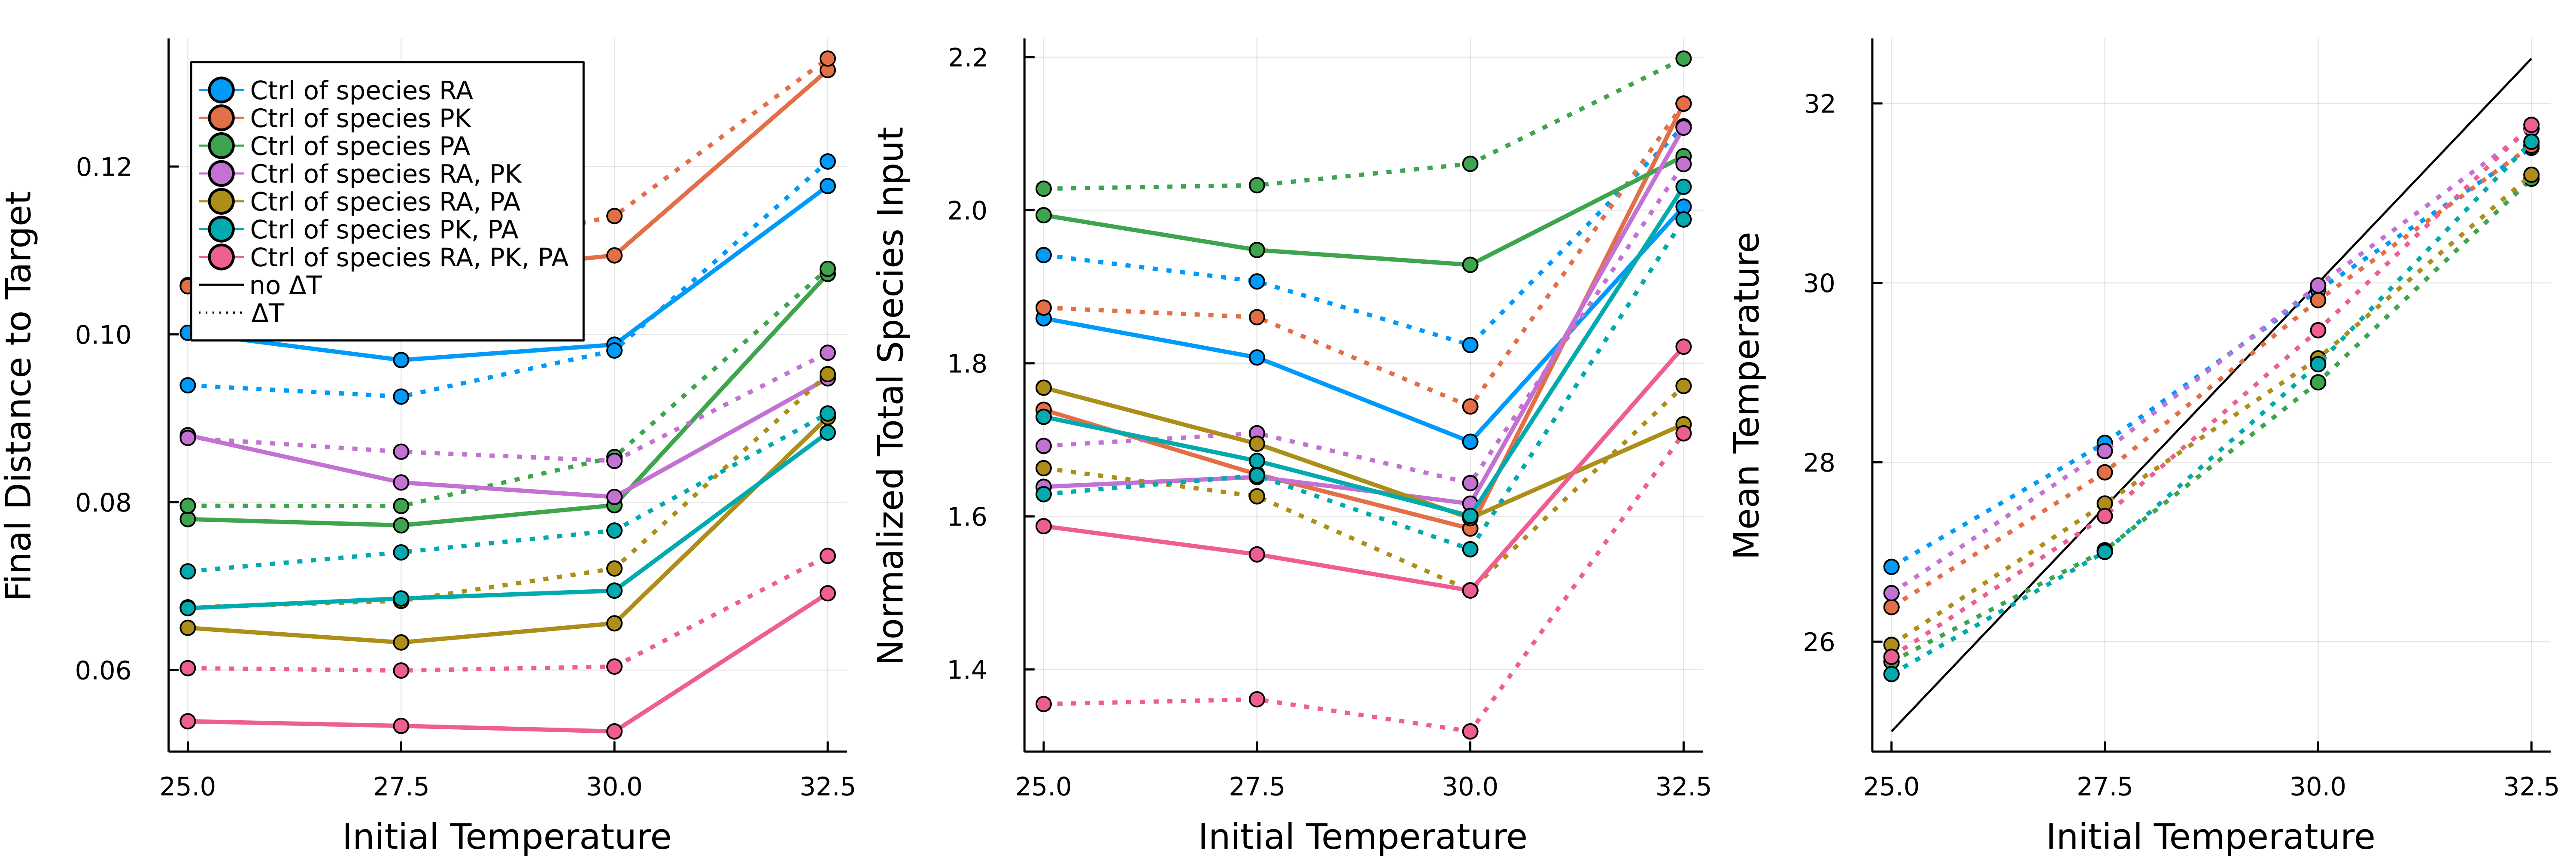
\includegraphics[width=2.0\columnwidth]{figs/MPC_Overall_Figure_allconfig.png}
    \centering
    \caption{\textbf{Summarized Success of MPC} Path and replicated averaged comparison of the linearized MPC with (dashed line) and without (solid line) the control of temperature for various sets of control species. (a) The final distance of the controller to the target equilibrium (b) The normalized, total species input in the control program (c) The mean temperature of the control program. }\label{fig:mpc_overall}
\end{figure*}

To explore this control scheme and the potential to modify temperature, the MPC is made to drive the state from each of the subcommunity equilibria to the others ten times, perturbed by random disturbances on each input (Figure \ref{fig:mpc_paths}). For each equilibrium-to-equilibrium path, all possible control species sets are tested and the depicted final species distance and total species input are averaged over all runs and sets. 

In both temperature controlled and fixed settings, the MPC is able to achieve closer final points with less input at lower temperatures on most paths regardless of input configuration. There are some exceptions such as when the MPC is driven to the RA-PA equilibria which the model depicts as strongly unstable at lower temperatures but becomes the dominating autonomous fixed point at 32.5 degrees celsius (as seen in the experiments). In comparison, with path-to-path variation, the effect of temperature control offers relatively little difference for the MPC. While there are slight improvements in final distance overall, the ability to transiently change the temperature in planning does not recover poor states on the given time span and planning horizon.

The path-based perspective demonstrates that, for a range of temperatures, the MPC is able to exploit changes in growth rates and interactions regardless of input configuration. This suggests that there are localized fluctuations in the autonomous dynamics of the microbial competition that might be wielded to reach the target diversity with minimal input.

\begin{figure*} \setlength\abovedisplayskip{0pt}
    % [!h]
% \centering
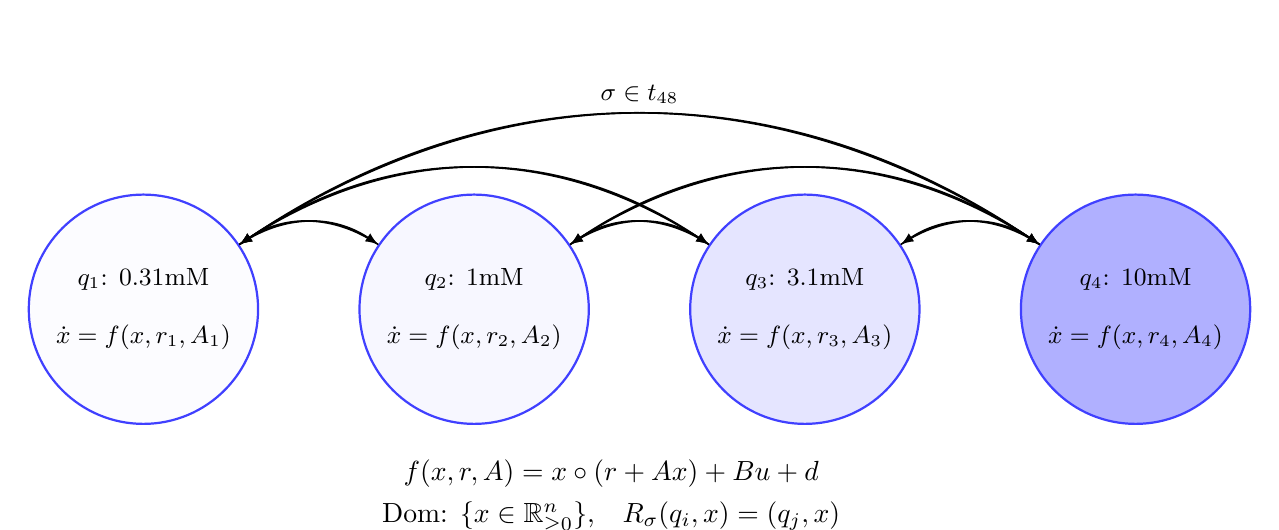
\begin{tikzpicture}[
    node distance=4.2cm,
    on grid,
    semithick,
    font=\small] 
 
% 0.31 mM   
\node
[ 
    state,
    fill=blue!1,
    align=center,
    inner sep=5pt
] (q_0) 
{
    $q_1$: $0.31$mM \\[10pt]
    $\dot{x}=f(x,r_{1},A_{1})$ 
};
% 1 mM   
\node
[
    state,
    fill=blue!3.1,
    align=center,
    inner sep=5pt
] (q_1) [right=of q_0] 
{
    $q_2$: $1$mM \\[10pt] 
    $\dot{x}=f(x,r_{2},A_{2})$ 
};
% 3.1 mM   
\node
[ 
    state,
    fill=blue!10,
    align=center,
    inner sep=5pt
] (q_2) [right=of q_1]
{
    $q_3$: $3.1$mM \\[10pt] 
    $\dot{x}=f(x,r_{3},A_{3})$ 
};
% 10 mM   
\node
[ 
    state,
    fill=blue!31,
    align=center,
    inner sep=5pt
] (q_3) [right=of q_2]
{
    $q_4$: $10$mM \\[10pt] 
    $\dot{x}=f(x,r_{4},A_{4})$ 
};
% Transitions
\path [-latex]
    (q_0) edge [bend left=34] 
        node [above] {} (q_1)
    (q_0) edge [bend left=34] 
        node [above] {} (q_2)
    (q_0) edge [bend left=34] 
        node [above] {$\sigma \in t_{48}$} (q_3)
    (q_1) edge [bend left=34] 
        node [above] {} (q_2)
    (q_1) edge [bend left=34] 
        node [above] {} (q_3)
    (q_2) edge [bend left=34] 
        node [above] {} (q_3)
    (q_1) edge [bend right=34] 
        node [above] {} (q_0)
    (q_2) edge [bend right=34] 
        node [above] {} (q_0)
    (q_3) edge [bend right=34] 
        node [above] {} (q_0)
    (q_2) edge [bend right=34] 
        node [above] {} (q_1)
    (q_3) edge [bend right=34] 
        node [above] {} (q_1)
    (q_3) edge [bend right=34] 
        node [above] {} (q_2);

\node [Mytext, below=of q_1, xshift=11.5ex, yshift=14ex] (f_lab) {\normalsize $f(x,r,A) = x \circ (r + Ax) + Bu + d$};
\node [Mytext, below=of f_lab, , yshift=24ex] {\normalsize Dom: $\{x \in \mathbb{R}^n_{\geq 0}\}$,\quad $R_\sigma (q_i,x)=(q_j,x)$};

\end{tikzpicture}
\end{figure*}

For an input-driven understanding of the effect of temperature control, the success of the MPC with a given control species set is averaged over all paths (Figure \ref{fig:mpc_overall}). Grouping by input configuration reveals that, regardless of temperature fluctuation, the more species that can be actuated, the better the system is controlled with closer final distances and more efficient input usage. Notably, this analysis illuminates that with more inputs, temperature control has an interesting ability to trade final point accuracy for normalized total input. In combination with the path-partitioned analysis, this implies that the benefit of temperature control can only be realized in an MPC with richer input configurations.

It is important to note that incorporation of temperature control does not force the MPC to change the temperature, and the trivial option of no temperature change is considered in the optimization problem. Hence, the deviation of the MPC with temperature control over the given horizon must have occurred because a change in temperature lowered the balanced cost between distance to target and sum input (\label{MPC_cost}). This suggests the tradeoff between final species distance and sum input in these experiments is a result of the relative sizes of the penalty matrices $Q$, and $R$ which could be altered to suit the designer. 

In cases, such as when only one species was actuated, where adding temperature control resulted in both a higher final species distance and sum input that we know the controller truly failed. Given that the trivial option of static temperature was considered, this failure can be traced back to two possible sources. First, there is the discrepancy between the linearized dynamics and the true parameter-varying gLV system, and its possible that over the horizon this error was exacerbated by the linearization of the polynomial, temperature-parameter relationship. In many cases though, the parameter variation was minimal or pseudo-linear. Second, the horizon size of the MPC ($n=5$) could've steered towards temperature domains yielding only short-term payoff (regardless of the dynamical approximation), particularly in the cautious problem outlined above with small input constraints. While raising the horizon comes at a computational cost, the slow dynamics of the gLV system would likely allow a user to exert grander search and optimization efforts in online action, ameliorating both the second and first issues. 

Overall, the MPC simulations demonstrated the usage of temperature introduced freedom in the modulation of the microbial community to reduce the efficiency of probiotic and antibiotic input by approximately $20\%$ at best at a sacrifice of $15\%$ final distance to target at worst. However, this was only available under the simple MPC employed with a fully actuated system. This option is still valuable considering the uncertainty surrounding probiotic and antibiotic inputs and the impressive raw final distance the MPC is able to achieve as is. This benefit may become more valuable if longer durations at these equilibria were required because the sum input will increase (despite final distance remaining constant) for the equilibria that are autonomously unstable. Finally, through fine-tuning of the optimization problem with real data, the addition of temperature control should perform equally at worst for all input configurations.

\subsection*{Hybrid Control of Glucose-Varying Systems}

\indent \indent Glucose is a complex environmental signal. As populations grow, the concentration of glucose falls in proportion to each population, hence, in reality the glucose dependent parameters are dependent on the total abundance and diversity. The fit proves that constant gLV parameters reasonably predict the dynamics on multi-hour intervals ie. that ecological pressures remain constant in this window, perhaps because of sensing delays facilitated by kinetic thresholds. However, to assume this would remain true for rapid fluctuations could be erroneous. If the interactions were majorly determined by delayed enzymatic repression and activation, sudden rises and falls in glucose concentration could induce more complex behavior, better represented by Hill terms rather than polynomials. For this reason, we consider the problem of driving microbiomes in glucose-varying models through a hybrid formulation, where each discrete $q$-state corresponds to a different set of parameters determined by the level of glucose introduced at restricted intervals,

% \begin{align*} \label{f_D_R}
%     \begin{array}{l}
%         f(x,r,A) = x \circ (r + Ax) + Bu + d \\
%         Dom: 
%     \end{array}
% \end{align*}

\noindent In addition to continuous state inputs $u$, the discrete action $\sigma$ of switching glucose-associated modes on 4-hour intervals is now possible. Each state shares the domain $Dom$ of the original model but unlike the experiments, the reset $R_\sigma$ associated with discrete state switching is the identity map (population dilutions might be unavailable in hydroponic culturing). 

We now define the optimal control problem as a zero-sum game between the controller and disturbance both subject to the system dynamics. The value function $J(x,t)$ of the game is determined by proximity to a target equilibrium $\bar{x}$,
\begin{equation}\label{Value}
    J(x,t) := \min_{u} \max_{d} \left\lVert x(t) - \bar{x} 
    \right\rVert
\end{equation}
\noindent thus, the controller is minimizing the distance to the equilibrium and takes the action for the worst possible disturbance. Given a window $t \in [\tau, 0]$, we seek the initial set of states $\mathcal{G}(\tau)$ for which the controller can drive to within an $\epsilon$ radius of $\bar{x}$ by $t=0$, 
\begin{equation}\label{BRT}
    \mathcal{G}(\tau) := \{ x | J(x, 0) < \epsilon \}
\end{equation}
\noindent also known as the Backwards Reachable Tube (BRT)[BRT-paper]. To compute the BRT, it is possible to solve the following Hamilton-Jacobi-Isaac's PDE for which $J(x,t)$ is a viscosity solution [[47] of BRT-paper],
\begin{equation}\label{HJI}
    -\frac{\partial J}{\partial t} = \min_{u} \max_{d} \frac{\partial J}{\partial x} \boldsymbol{\cdot} f(x, u, d)
\end{equation}
\noindent While the exact solution to this PDE is unknown in general, it is possible to obtain a numerical approximation for the level set of $\mathcal{G}(\tau)$ by gridding a subspace of $\mathbb{R}^n$ and recursively evaluating the change in $J$ over time [Mo, Ian]. These computations are accelerated with the Python toolbox OptimizedDP [Mo Chen].

We compute and compare the BRT of the RA-PK-PA equilibrium under fixed environments with environments subjected to scheduled switching. While the data showed this equilibrium is autonomously stable, we include this target to gauge how environmental control can change the rate of convergence. For the static environment, we compute the BRT with $\tau = -12$ hours for each of the four hybrid states corresponding to the glucose concentrations, and in the switched environment, we iteratively compute the BRT of $\tau = -4$ hour segments in which the target set becomes the previous BRT computation, for all $4^3$ possible switch schedules. 

\begin{figure}[!ht]
    \centering
    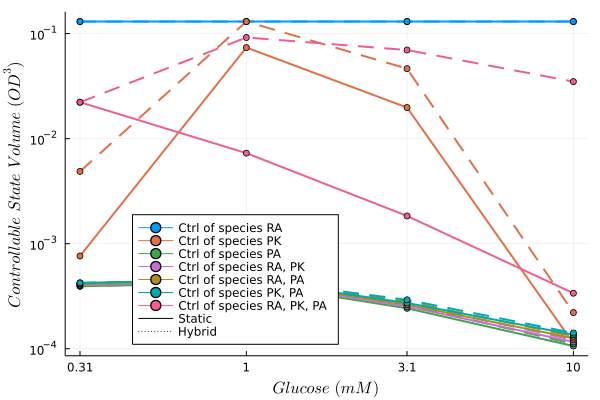
\includegraphics[width=1.0\columnwidth]{figs/BRT_comp.png}
    \centering
    \caption{\textbf{Comparison of BRT Volumes for Static and Switched Environments} The computed controllable state volume of the static environment problems (solid line) along with the hybrid schedule resulting in maximum volume (dashed line) for each of the glucose concentrations. }\label{fig:hs_vr}
\end{figure}

\begin{figure*}[!ht]
    \centering
    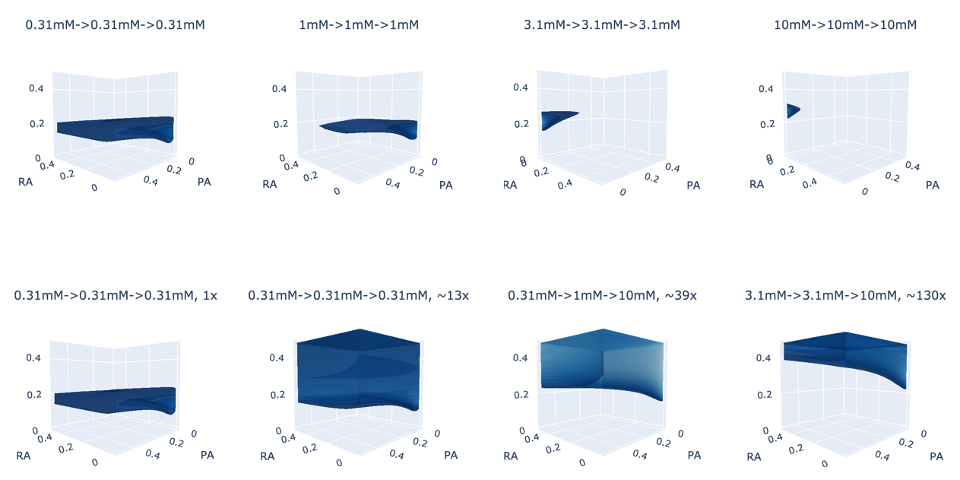
\includegraphics[width=2.0\columnwidth]{figs/all_BRT.png}
    \centering
    \caption{\textbf{Backwards Reachable Tubes of Hyrbid Glucose HJI Control} Each column corresponds to the comparison of the fixed environment BRT (top) and maximum hybrid BRT (bottom) for driving to the fixed environment's RA-PK-PA equilibrium. The relative size of the maximum volume is listed in its title. }\label{fig:hs}
\end{figure*}

The comparison of controllable state volumes for static and hybrid glucose environments is plotted for all control configurations (Figure \ref{fig:hs_vr}). A couple trends are noticeable from these plots. For some input configurations, including all two member control species sets, the computed BRT is small and minimally variant with switched or static environments suggesting uncomprimising dynamics (bug with these runs in trying to turn off input?). Alternatively, in the case with control over only species RA, the entire searched state space falls within the BRT, and we will have success with or without switched environments. Finally, there are mixed outcomes which demonstrate a significant increase in the size of controllable space. Generally, this reiterates an underlying trend in the virtual MPC runs that intermediate concentrations of glucose yield the most manageable system dynamics.

Similar to the virtual experiments with the MPC, we observe the greatest benefit of environment-variation when its possible to actuate all species. We can interrogate this phenomenon through direct observation of the BRT surfaces: for each glucose concentration and it's corresponding RA-PK-PA equilibrium, the static environment BRT and the maximum volume BRT of all possible switched schedules are juxtaposed (Figure \ref{fig:hs}).

As the static environment is the trivial schedule of switching to itself, the maximum BRT must be greater than or equal to the static BRT, however, we observe maximum volumes up to $130x$ greater. Notably, the maximum volume switched BRT includes utilizing the dynamics of lower glucose systems for at least two of the switches in all cases despite the previous analyses which revealed these systems to have the slowest rates of convergence. With respect to the dynamics and the previous analyses, we interpret this outcome as a product of more efficient and effective input due to more amenable interactions in the lower environment ranges. When the glucose concentration is lower, attenuated growth of PA in particular must allow for the freedom to traverse a greater range of diversities. Ultimately, if it were necessary to rapidly converge to the autonomous RA-PK-PA equilibrium, potentially from a pairwise, isogenic or input-stabilized fixed point, it would be wise to maintain a glucose-constrained environment and in general, we can compute the optimal schedule for hyrbid gLV system given an initial point and a desired diveristy.

How can this make sense in comparison with the known phenomenon that stressed crops release rhizospheric glucose along with several other carbohydrates? Perhaps, this underscores the inverse interest of the plant under duress to select against diversity. While, a farmer may come to know healthy configurations of organisms for high yields, a noncognisant plant might have the most likely survival by choosing one major member and eradicating all other abundances and potentially a disease-causing member.

\section*{Conclusion}

The results of the experimental work further supports the high-resolution parameterization method proposed by Venturelli et al. and demonstrates that variations in these parameters due to the environment are also predictable by the gLV system. This implies that gLV parameters are malleable in predictable ways under certain circumstances, perhaps with well fit models and small deformations. Practically, this knowledge is valuable for assessing how a community, designed or natural, might fluctuate under perturbations of the environment due to season, stress or design, and what might be the dominating diversity in such situations. Notably, the modelling illuminated the variance in rates of convergence in different environments. In future work, we hope to interrogate how the observed parameter variations compare to those of other environmental disturbances and those of the same disturbances on other communities. We are unable to answer why glucose and temperature induced such similar fluctuations of dynamics and would like to explore if there exists a general variational pattern under arbitrary stress for this and other microbial communities.

The theoretical control of parameter-varying gLV systems demonstrated that knowledge of environmental dependence can be valuable when modulating a micriobiome. In general, the simulations underscored that certain environments are more amenable to altering a community, inversely correlated with rates of convergence. Moreover, they demonstrated that controlling the environment can improve modulation programs by finding more optimal paths - in terms of final distance to target diversities and total input - and by increasing the set of controllable states under certain input configurations. This is likely to be related to the interaction network configuration and the minimal driver species, however, this analysis yielded inconclusive results for the parameter networks here (not shown). The control theoretic findings were ultimately promising but  nuanced. Under stringently controllable systems more sophisticated algorithms will be necessary to take advantage of induced variations in competition, perhaps by advanced numerical methods or reinforcement learning [michael and ben], and we leave this to future work.

In summary, these experiments, in vitro and silico, demonstrated how environment-dependent competitive dynamics within the soil microbiome can be modeled by parameter-varying gLV systems and that this knowledge can be valuable for improving control of these systems. Both of these findings offer new directions for deisgning and controlling microbial communities in human health, agriculture and chemical production.

\section*{Acknowledgements}

We would like to thank Adam Deutschbauer and Hans Carlson for their counsel and assisstance in the pooled sequencing of all pairwise and triwise experiments. We would like to thank Morgan Price for his Perl scripts for analyzing the pooled sequencing results. We would like to thank Claire Tomlin and Shankar Deka for valuable discussions on Model Predictive and Hamilton-Jacobi controllers.

\section*{References (In progress)}

1. Rosenbaum, Michael, Rob Knight, and Rudolph L. Leibel. "The gut microbiota in human energy homeostasis and obesity." Trends in Endocrinology \& Metabolism 26.9 (2015): 493-501.

2. Lyte, Mark. "Microbial endocrinology and the microbiota-gut-brain axis." Microbial endocrinology: the microbiota-gut-brain axis in health and disease (2014): 3-24.

3. Johnson, Katerina V-A., and Kevin R. Foster. "Why does the microbiome affect behaviour?." Nature reviews microbiology 16.10 (2018): 647-655.

4. Lakshmanan, Venkatachalam, Prasun Ray, and Kelly D. Craven. "Toward a resilient, functional microbiome: Drought tolerance-alleviating microbes for sustainable agriculture." Plant Stress Tolerance. Humana Press, New York, NY, 2017. 69-84.

5. Venturelli, Ophelia S., et al. "Deciphering microbial interactions in synthetic human gut microbiome communities." Molecular systems biology 14.6 (2018): e8157.

6. Bucci, V., Tzen, B., Li, N. et al. MDSINE: Microbial Dynamical Systems INference Engine for microbiome time-series analyses. Genome Biol 17, 121 (2016). https://doi.org/10.1186/s13059-016-0980-6

7. Clark, Ryan L., et al. "Design of synthetic human gut microbiome assembly and butyrate production." Nature communications 12.1 (2021): 1-16.

Angulo: A theoretical Framework for controlling complex microbial communities

Liu: Controlling complex networks

Justice, Nicholas B., et al. "Environmental selection, dispersal, and organism interactions shape community assembly in high-throughput enrichment culturing." Applied and environmental microbiology 83.20 (2017): e01253-

Gore Dilution: https://dspace.mit.edu/bitstream/handle/1721.1/128220/journal.pcbi.1007934.pdf?sequence=2\&isAllowed=y

Borreli: Hybrid MPC formulations

Tomlin: Backwards Reachable Tube paper?
https://arxiv.org/pdf/1709.07523.pdf

Michael and Ben 

\section*{Supplemental (In progress)}

\begin{figure*}[!ht]
    \centering
    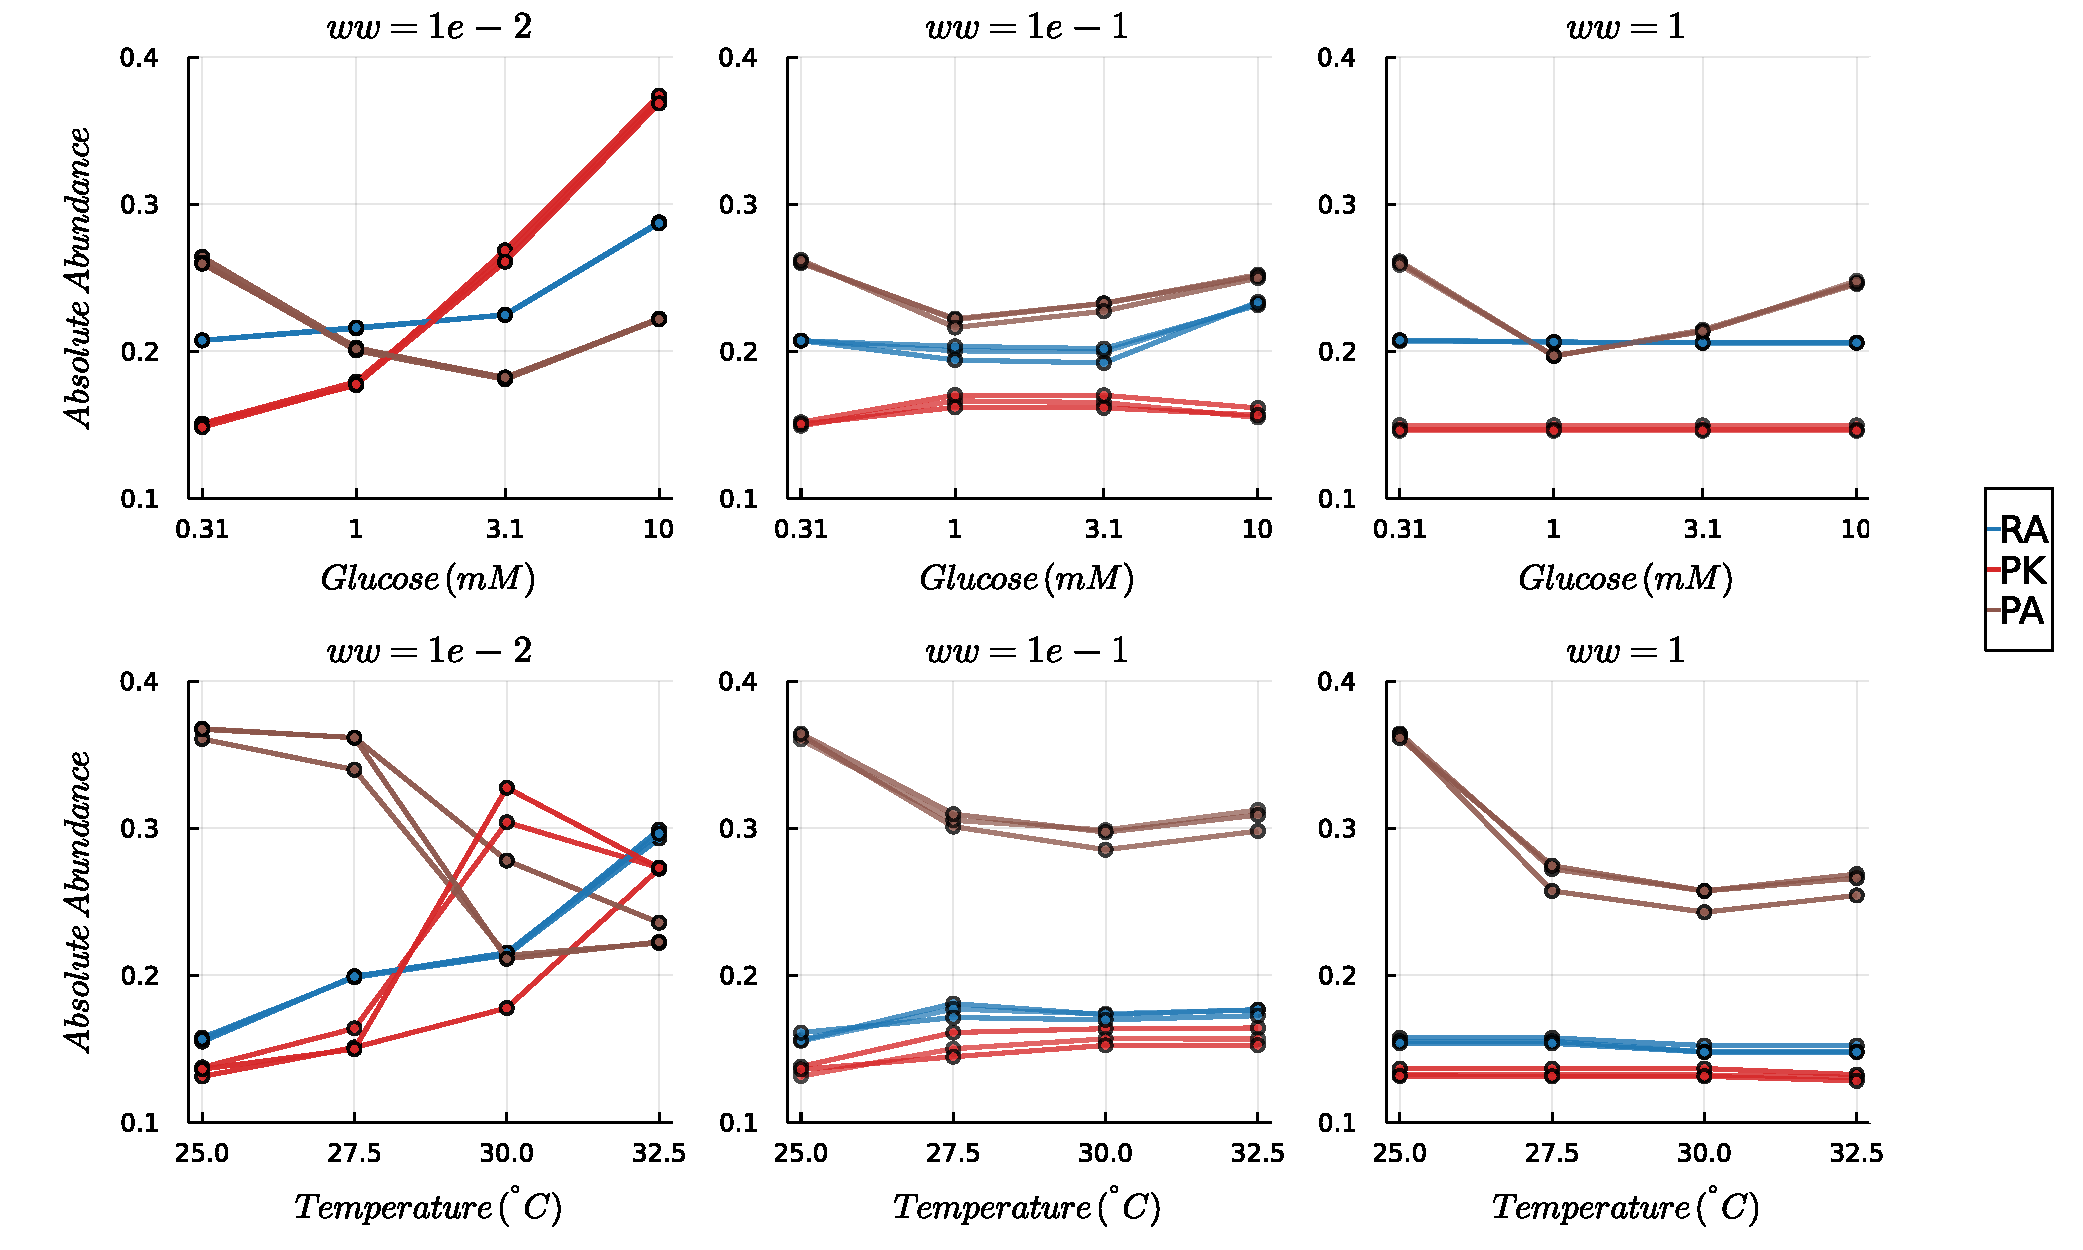
\includegraphics[width=2.0\columnwidth]{figs/isoabun_over_wwfits.pdf}
    \centering
    \caption{\textbf{Interaction Variance over Model Ensemble} Three parameter outputs of the optimization algorithm are displayed for three different wander regularization penalties for both glucose and temperature settings. }\label{fig:iv}
\end{figure*}

\begin{enumerate}
    \item \textcolor{ForestGreen}{Figure on PCA of gLV fits with and without the wander weight?}
    \item \textcolor{ForestGreen}{Figure of Fangchao direct pcr vs. qiagen results}
    \item \textcolor{ForestGreen}{Figure of Sensitivities of Best Fit}
\end{enumerate}

% \end{multicols}

\end{document}

%% Things remaining to do: %%

-- modeling:
 - Use gradient descent to optimize the evo opt of base (first itself than for each)
    - if c == 1 or 5, gradient descent on self with self data
    - else do gradient descent on c-1 with self data (follow up on gitter and julialang posts)

 - sensitivity analysis over ensemble to identify which p even matter (p-mean and std, p-sens-mean and std)

 - with ensemble of models and relevant p, make solid interpretations of 
    - interaction changes 
    - fixed point & stability, due to limit cycle

-- control:
 - find bug in mpc graph plot
    - finish MPC writing once this is concluded (not hard)

- write conclusion

- formalize references 

- plot hybrid vs static BRT volumes np data in julia

% The gLV model can be used to study the network of interactions in the microbiome with adjacency matrix $A$. Weighted ecological networks often appear to be complete graphs [Venturelli, Bucci], however, it is rare to parameterize an interaction coefficient to $0$ exactly; numerical optimization of the gLV model is nuanced. To discuss the change in graph density and connectivity, we might limit consideration to edges above a minimum absolute value. When identifying minimal driver species, Angulo et al. note that adding additional edges does not create autonomous elements, and in general, a more connected graph is likely to require fewer input nodes for controllability. Therefore, thresholding interactions at a higher minimum strength will assume a more cautious position. If a controlled graph were to depend on weak interactions for structural accessibility, input might become bottle-necked from driver species nodes to the end of all species nodes. We compare the change in density, connectivity and minimal driver species with respect to environment of the synthetic community for all interactions ($min( \lvert \alpha \rvert) > 0$), most interactions ($min( \lvert \alpha \rvert) > 0.5$), and strong interactions ($min( \lvert \alpha \rvert) > 1$) [Figure Networks].



